\documentclass{beamer}
\usepackage{beamerthemesplit}
\usepackage{pgfgantt}
\usetheme{Warsaw}
\usecolortheme{wolverine}
\usepackage{sidecap}
\usepackage[frenchb]{babel}
%\usepackage[latin1]{inputenc}
\usepackage[utf8x]{inputenc}
\usetikzlibrary{babel}
\usepackage[T1]{fontenc}
\usepackage{amsfonts}
\usepackage{amsmath,amssymb,mathrsfs,theorem}
\usepackage[all]{xy}
\usepackage{textcomp}
\usepackage{variations}
%\usepackage[framed,amsmath,thmmarks]{ntheorem}
\usepackage{pgfgantt}
\usepackage{animate}
\usepackage{pstricks,pst-plot,pstricks-add}
\usepackage{bm, ulem, listings, ccaption}
\usepackage{color, xcolor,epic,eepic,multicol,graphicx}
\graphicspath{{../Images_Fichiers/}}
\lstset{		language=Java,
 				backgroundcolor=\color{black},
                basicstyle=\color{white}\small,
                keywordstyle=\color{orange}\ttfamily,
                stringstyle=\color{olive}\ttfamily,
                commentstyle=\color{gray}\ttfamily,
                morecomment=[s][\color{lime}]{/**}{**/},
                keepspaces=true,
                morekeywords={module, export, constructor, let, of, number}, 
                showstringspaces=false, 
                tabsize = 2,
                morekeywords={[2]taille, choix, nbIterations, geo, position, links, to, hashNumber, x, y, z}, 
                keywordstyle={[2]\color{attributs}},
                morekeywords={[3]go, goForTheFirstTime, getValue, allKeys, putValue, tan, angleBetweenTwoVectorsBetween0andPi, newFrom, substract, min, max, add, scale, push, setPosition },
                keywordstyle={[3]\color{yellow}}, 
                morekeywords={[4]0, 1, 2, 3, 4, 5, 6, 7, 8, "9"}, 
                keywordstyle={[4]\color{blue}}
}
\newcommand{\gs}[1]{\textbf{\underline{#1}}}
\newcommand{\Z}{\mathbb{Z}}
\newcommand{\R}{\mathbb{R}}
\newcommand{\Q}{\mathbb{Q}}
\newcommand{\N}{\mathbb{N}}
\newcommand{\D}{\mathbb{D}}
\newcommand{\C}{\mathbb{C}}
\title{Les surfaces minimales}
\subtitle{Stage M1 - été 2017 }
\author{GRAFF Jonathan}
\date{\today}
\begin{document}
\maketitle

\AtBeginSection[]{
  \begin{frame}{Sommaire}
  \begin{columns}[t]
  \begin{column}{5cm}
  \tableofcontents[sections={1-2}, currentsection, currentsubsection, hideothersubsections]
  \end{column}
  \begin{column}{5cm}
  \tableofcontents[sections={3-4}, currentsection, currentsubsection, hideothersubsections]
  \end{column}
  \end{columns}
\end{frame}
}

\AtBeginSubsection[]{
  \begin{frame}{Sommaire}
  \tableofcontents[sections=\thesection{}, subsectionstyle=show/shaded/hide, subsubsectionstyle=show/show/hide]
 
\end{frame}
}

\begin{frame}{Sommaire}
  \begin{columns}[t]
  \begin{column}{5cm}
  \tableofcontents[sections={1-2}, pausesections]
  \end{column}
  \begin{column}{5cm}
  \end{column}
  \end{columns}
\end{frame}

\begin{frame}{Sommaire}
  \begin{columns}[t]
  \begin{column}{5cm}
  \tableofcontents[sections={1-2}]
  \end{column}
  \begin{column}{5cm}
  \tableofcontents[sections={3-4}, pausesections]
  \end{column}
  \end{columns}
\end{frame}


\section{Introduction} 

\begin{frame}
\frametitle{Les surfaces minimales :}
$\bullet$ se rencontrent dans la nature (films savonneux)\\
\begin{figure}[h!]
  \begin{minipage}[b]{0.40\linewidth}
    \centering 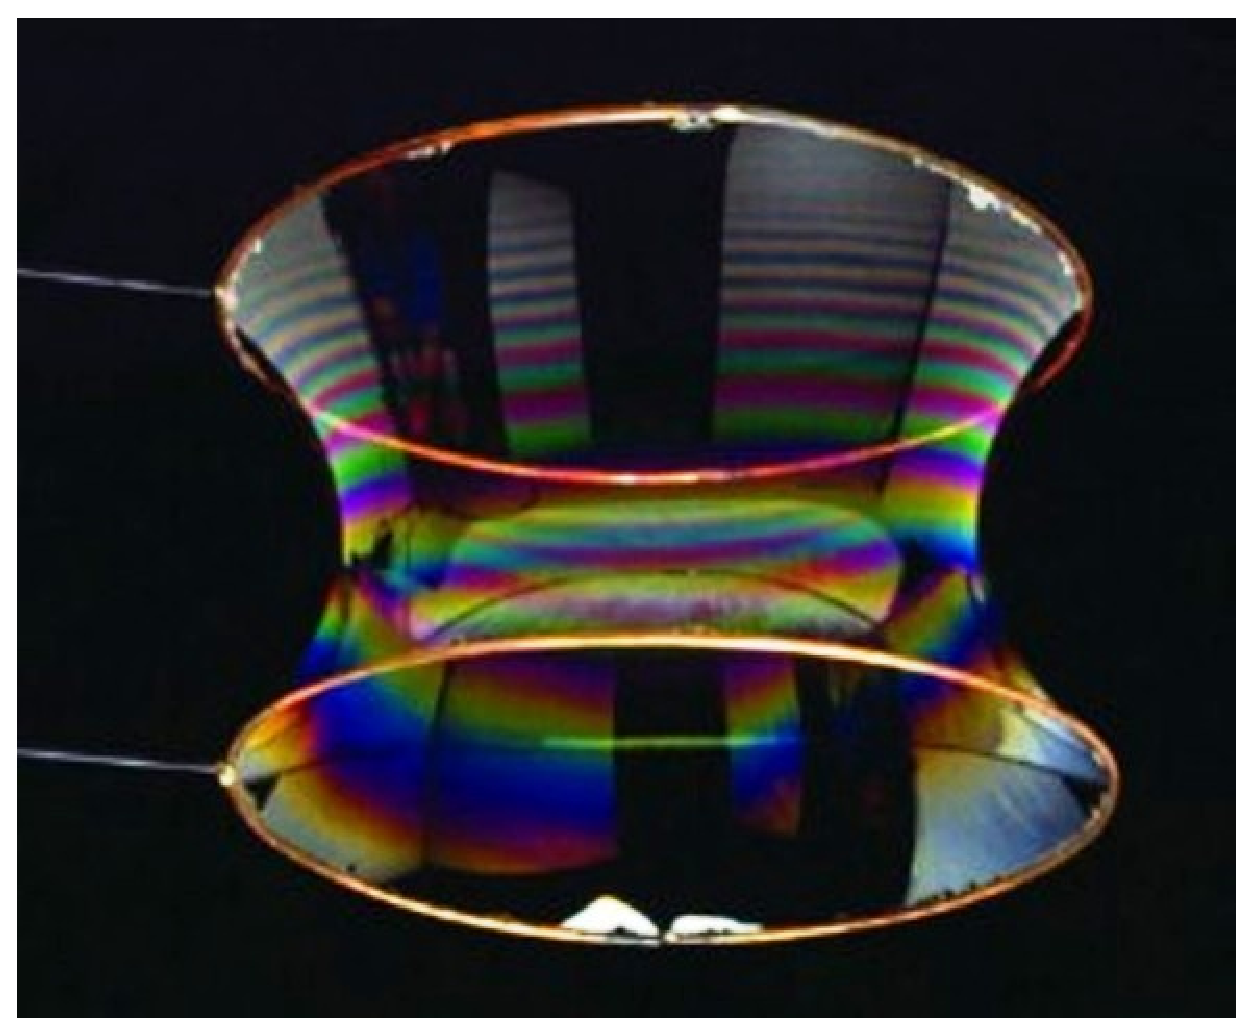
\includegraphics[scale=0.16]{savoncaten.eps}
 \end{minipage}
\begin{minipage}[b]{0.48\linewidth}   
 \centering 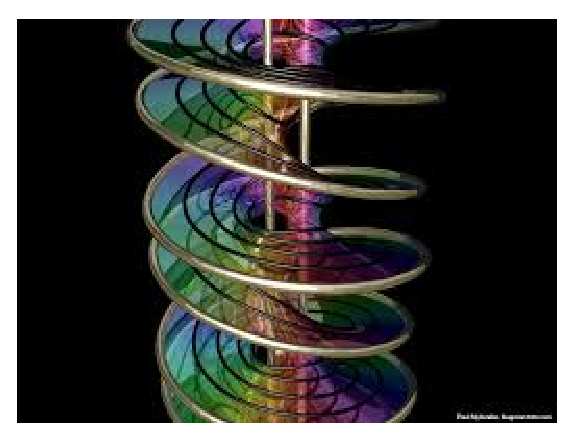
\includegraphics[scale=0.4]{savonhelico.eps}
\end{minipage}
\end{figure}
\begin{figure}[h!]
  \begin{minipage}[b]{0.40\linewidth}
    \centering 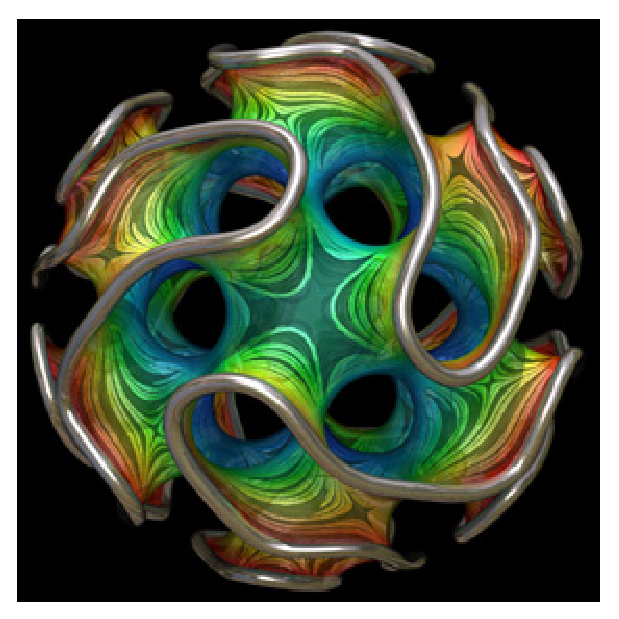
\includegraphics[scale=0.3]{savongyroid.eps}
 \end{minipage}
\begin{minipage}[b]{0.48\linewidth}   
 \centering 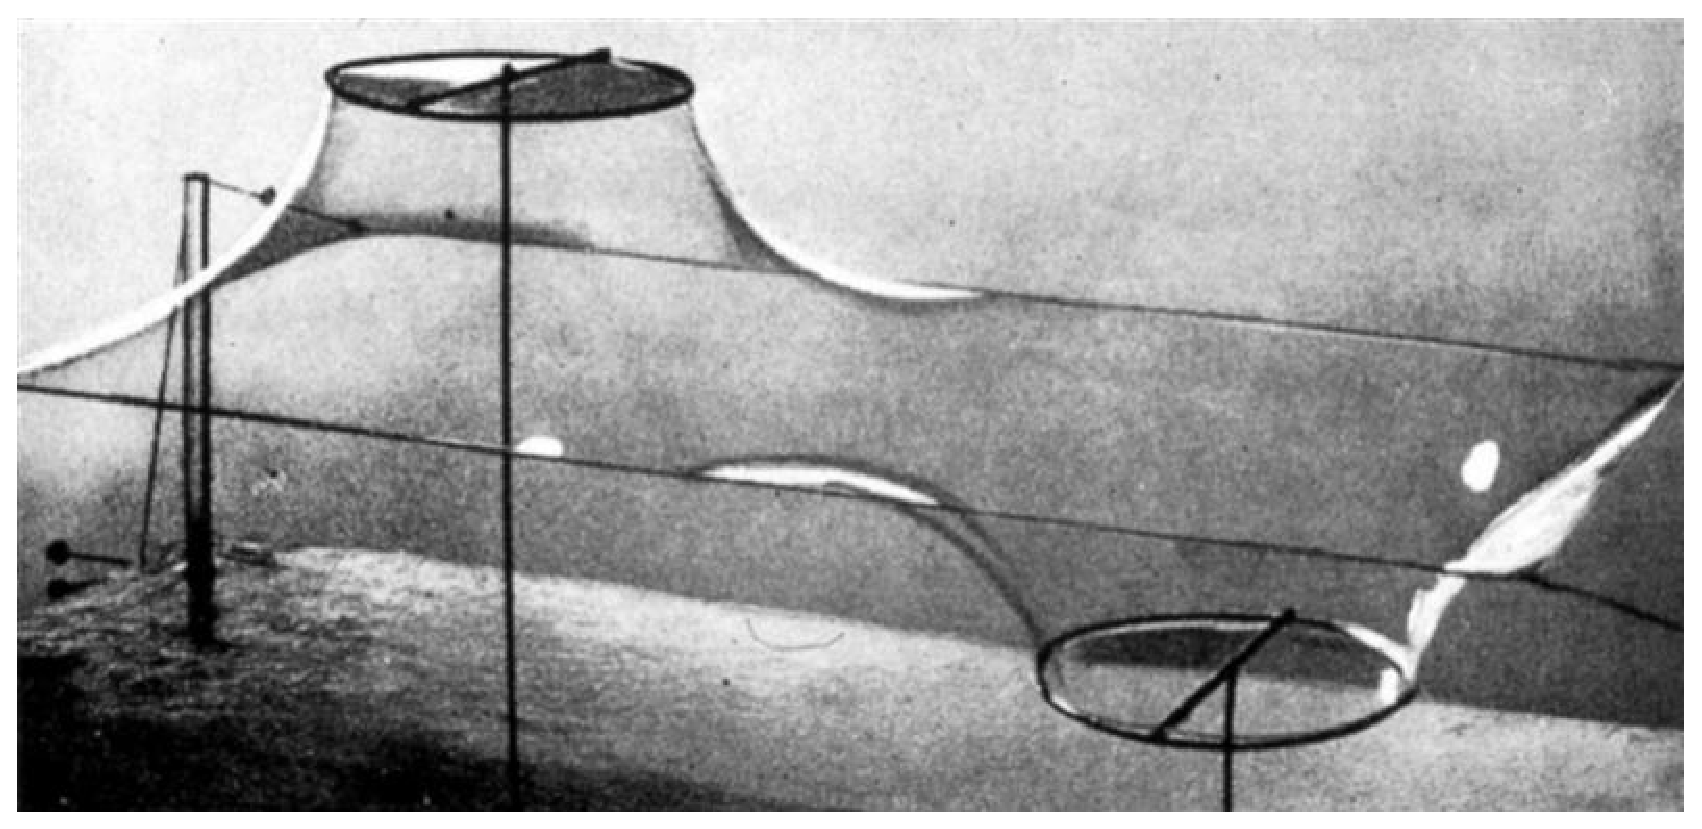
\includegraphics[scale=0.23]{savonriemann.eps}
\end{minipage}
\end{figure}
\end{frame}

\begin {frame}
\frametitle{Les surfaces minimales}
$\bullet$ sont utiles en physique, mécanique, architecture, pour minimiser des forces, des surfaces de frottements...\\
\pause 
$\bullet$ sont tout simplement jolies, et donc utilisées dans certains ouvrages d'art : \\
\pause
Le toit du stade olympique de Munich :
\begin{figure}[h!]
   \begin{minipage}[b]{0.45\linewidth}
      \centering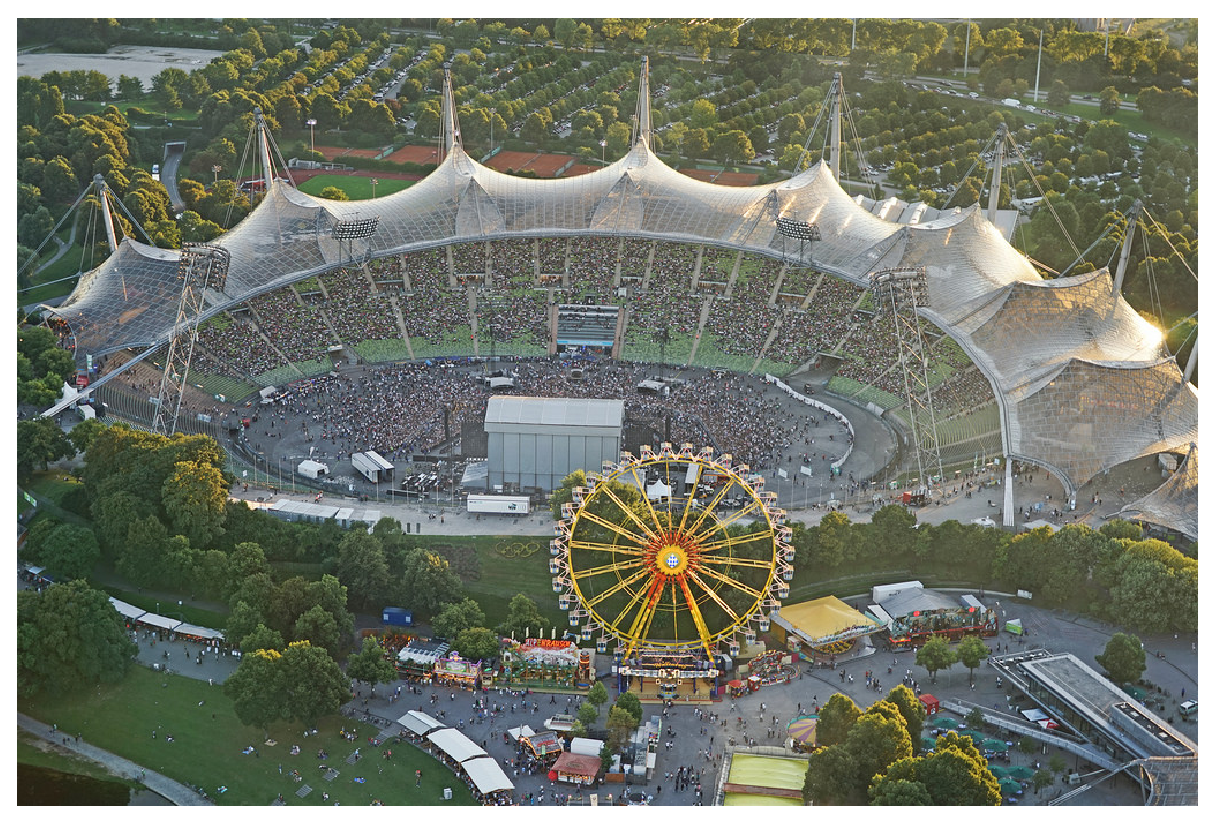
\includegraphics[scale=0.25]{stade1.eps}
   \end{minipage}
    \begin{minipage}[b]{0.50\linewidth}   
     \centering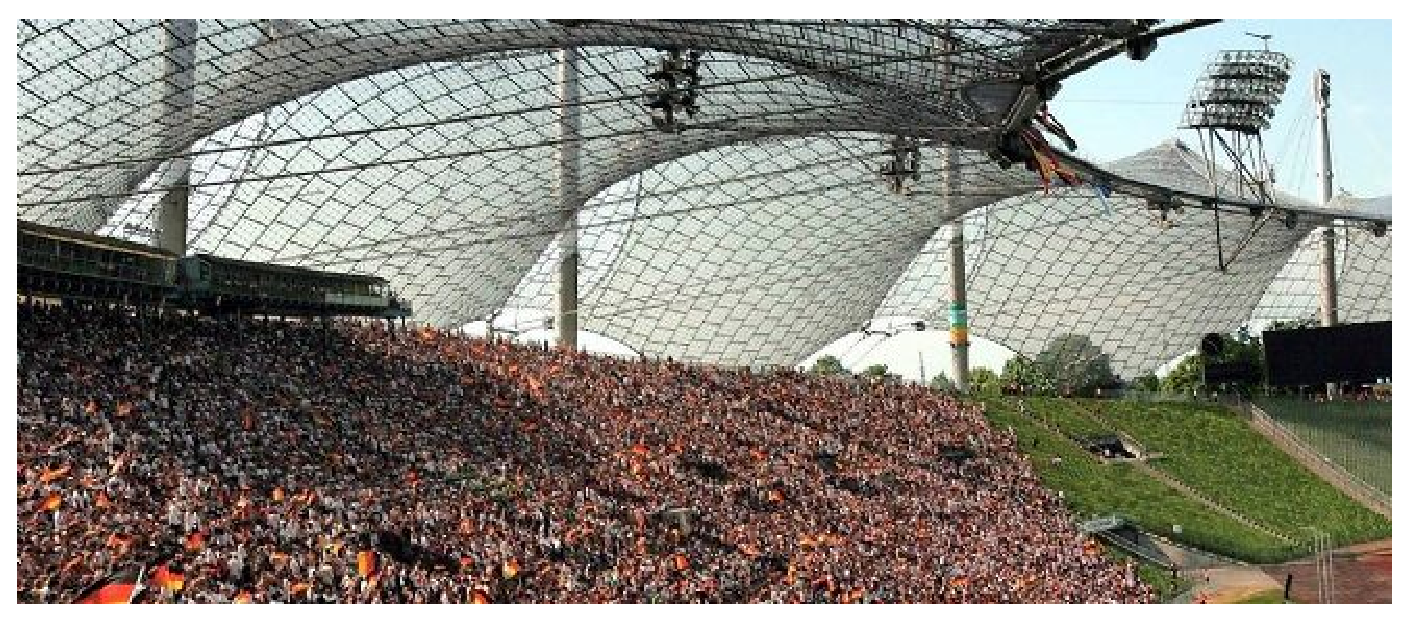
\includegraphics[scale=0.30]{stade2.eps}
   \end{minipage}
\end{figure}
\end {frame}

\begin {frame}
\frametitle{Oeuvres d'art}
\begin{figure}[h!]
   \begin{minipage}[b]{0.45\linewidth}
      \centering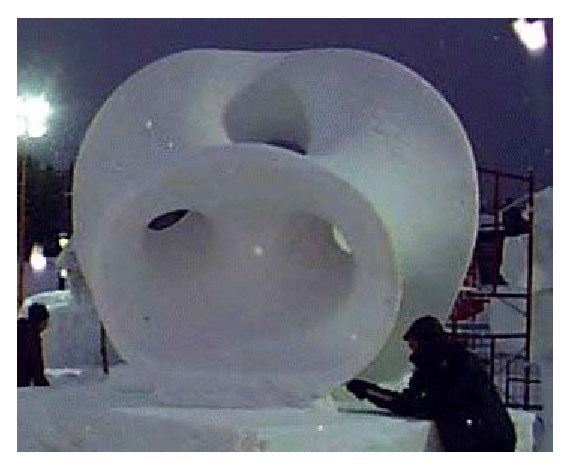
\includegraphics[scale=0.45]{costaice.eps}
   \end{minipage}
    \begin{minipage}[b]{0.50\linewidth}   
     \centering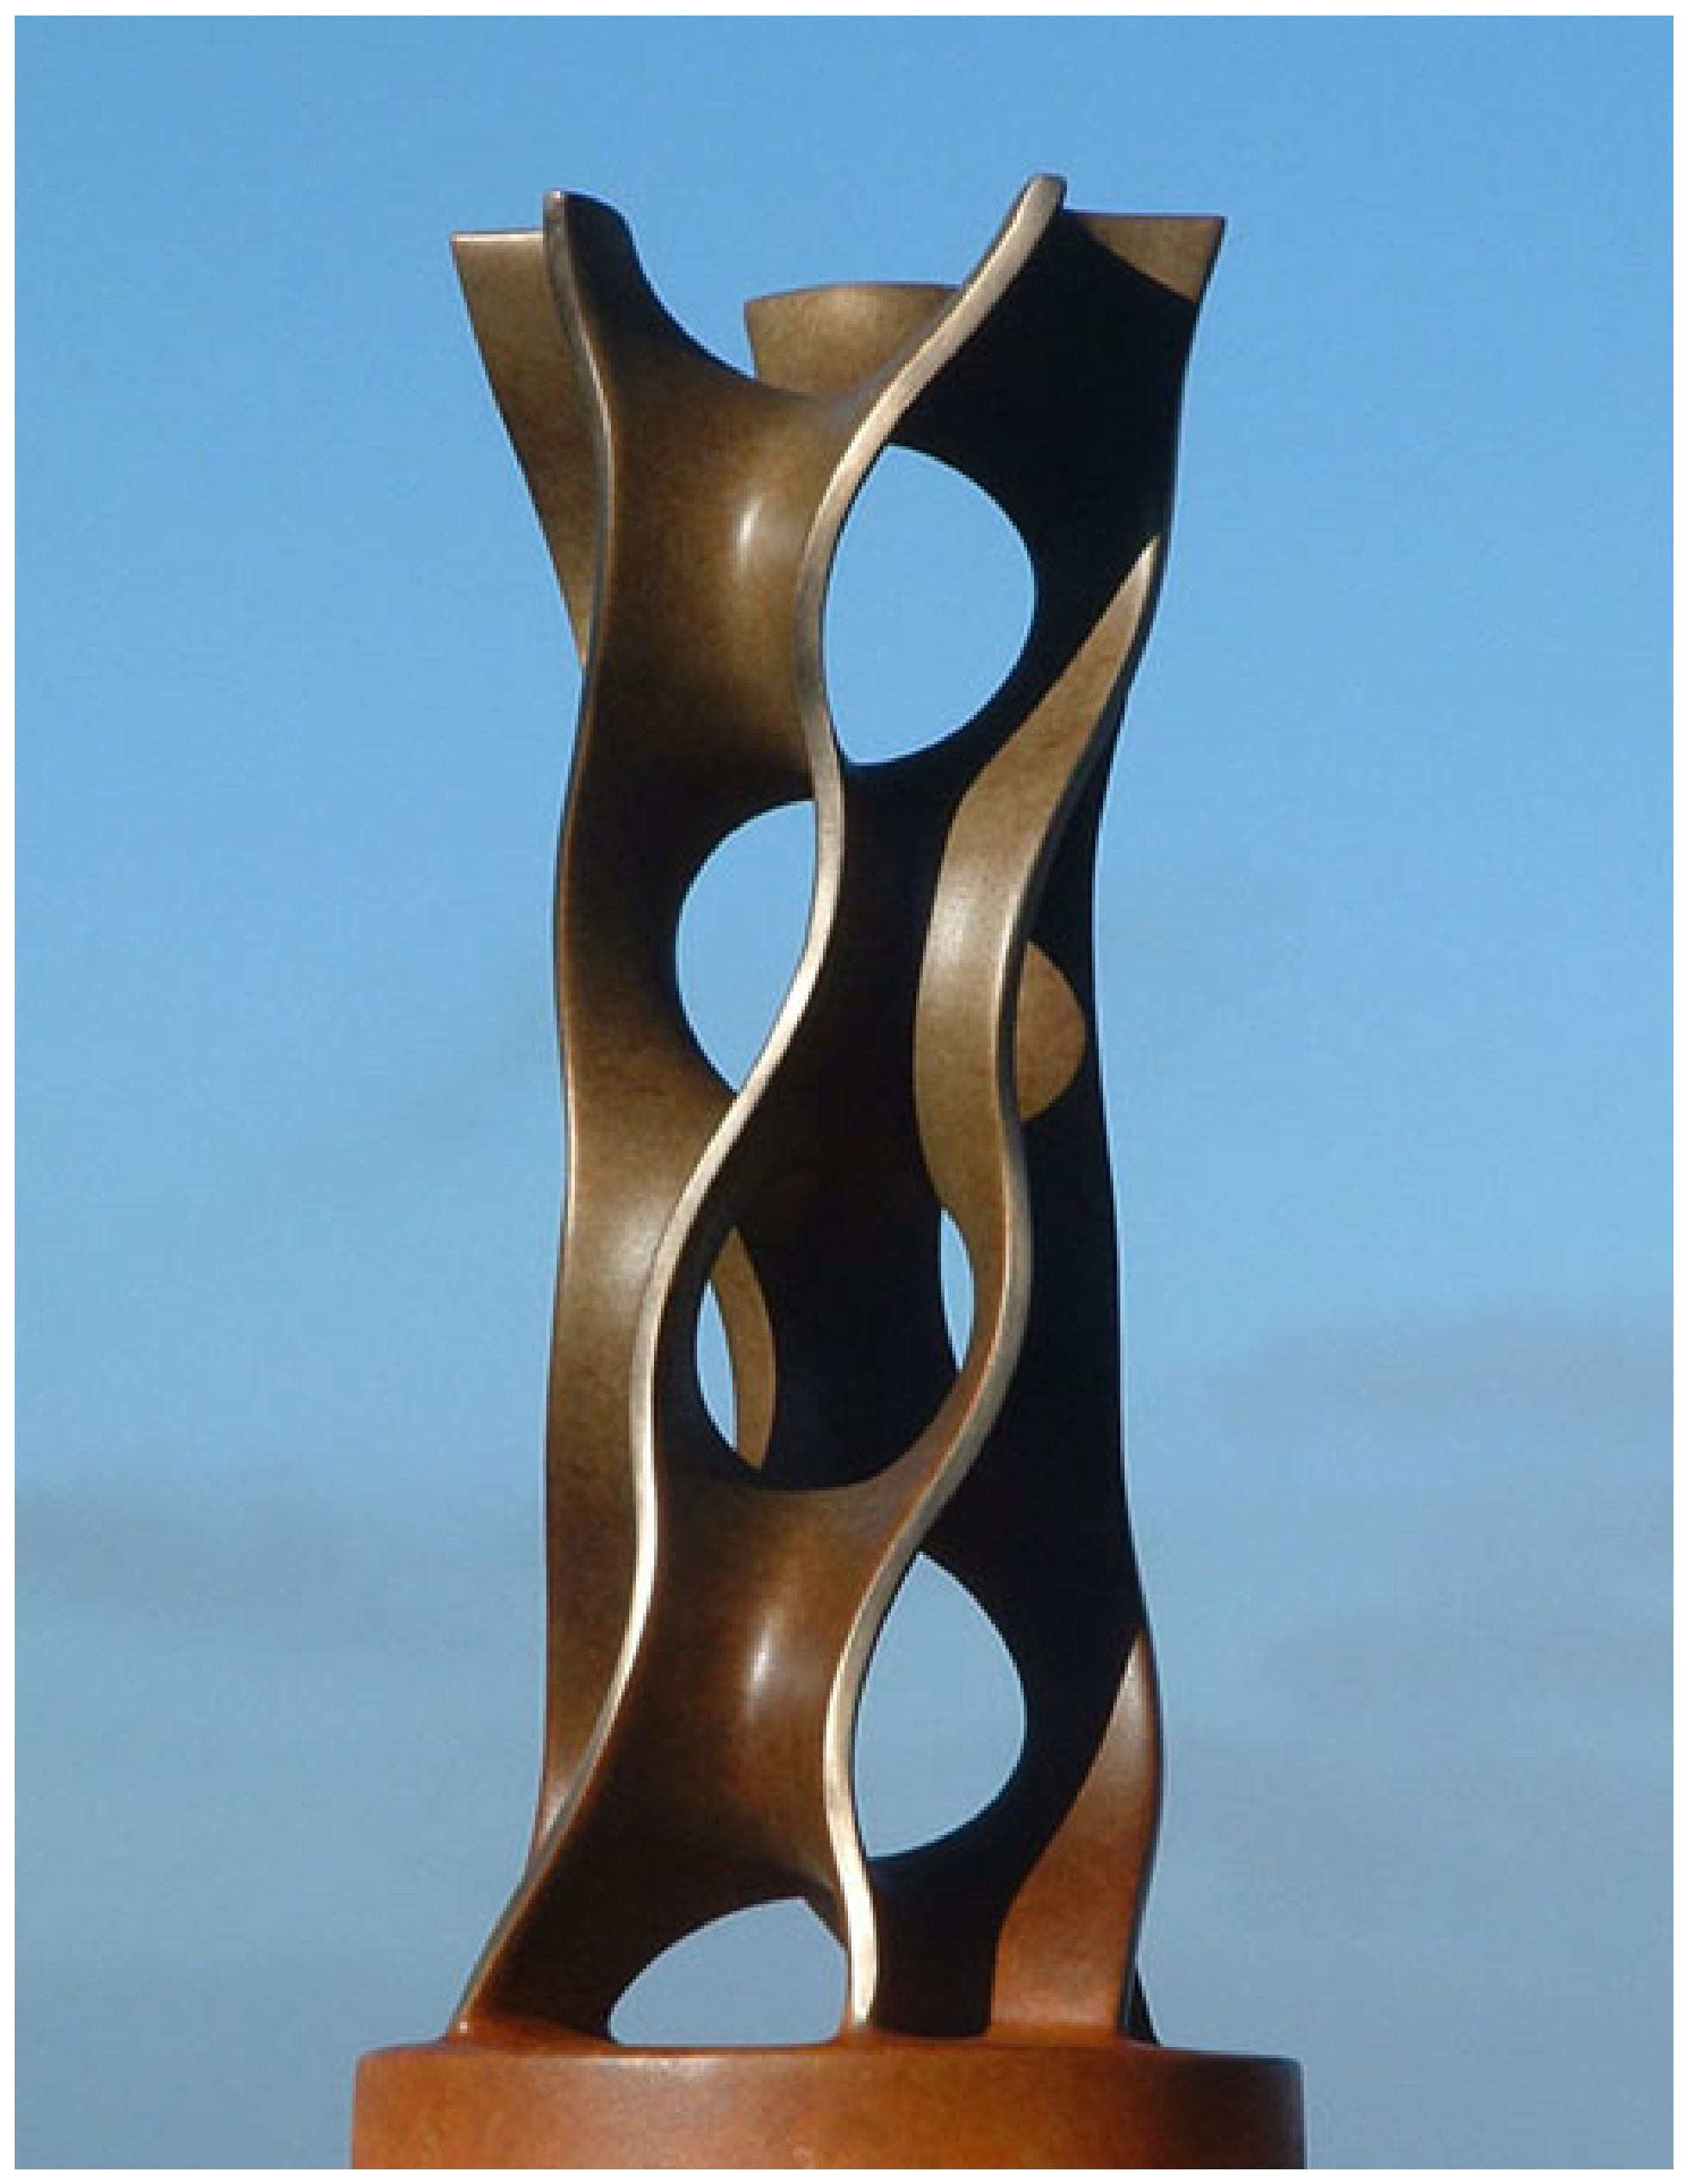
\includegraphics[scale=0.08]{scherktower.eps}
   \end{minipage}
\end{figure}
\begin{figure}[h!]
   \begin{minipage}[b]{0.45\linewidth}
      \centering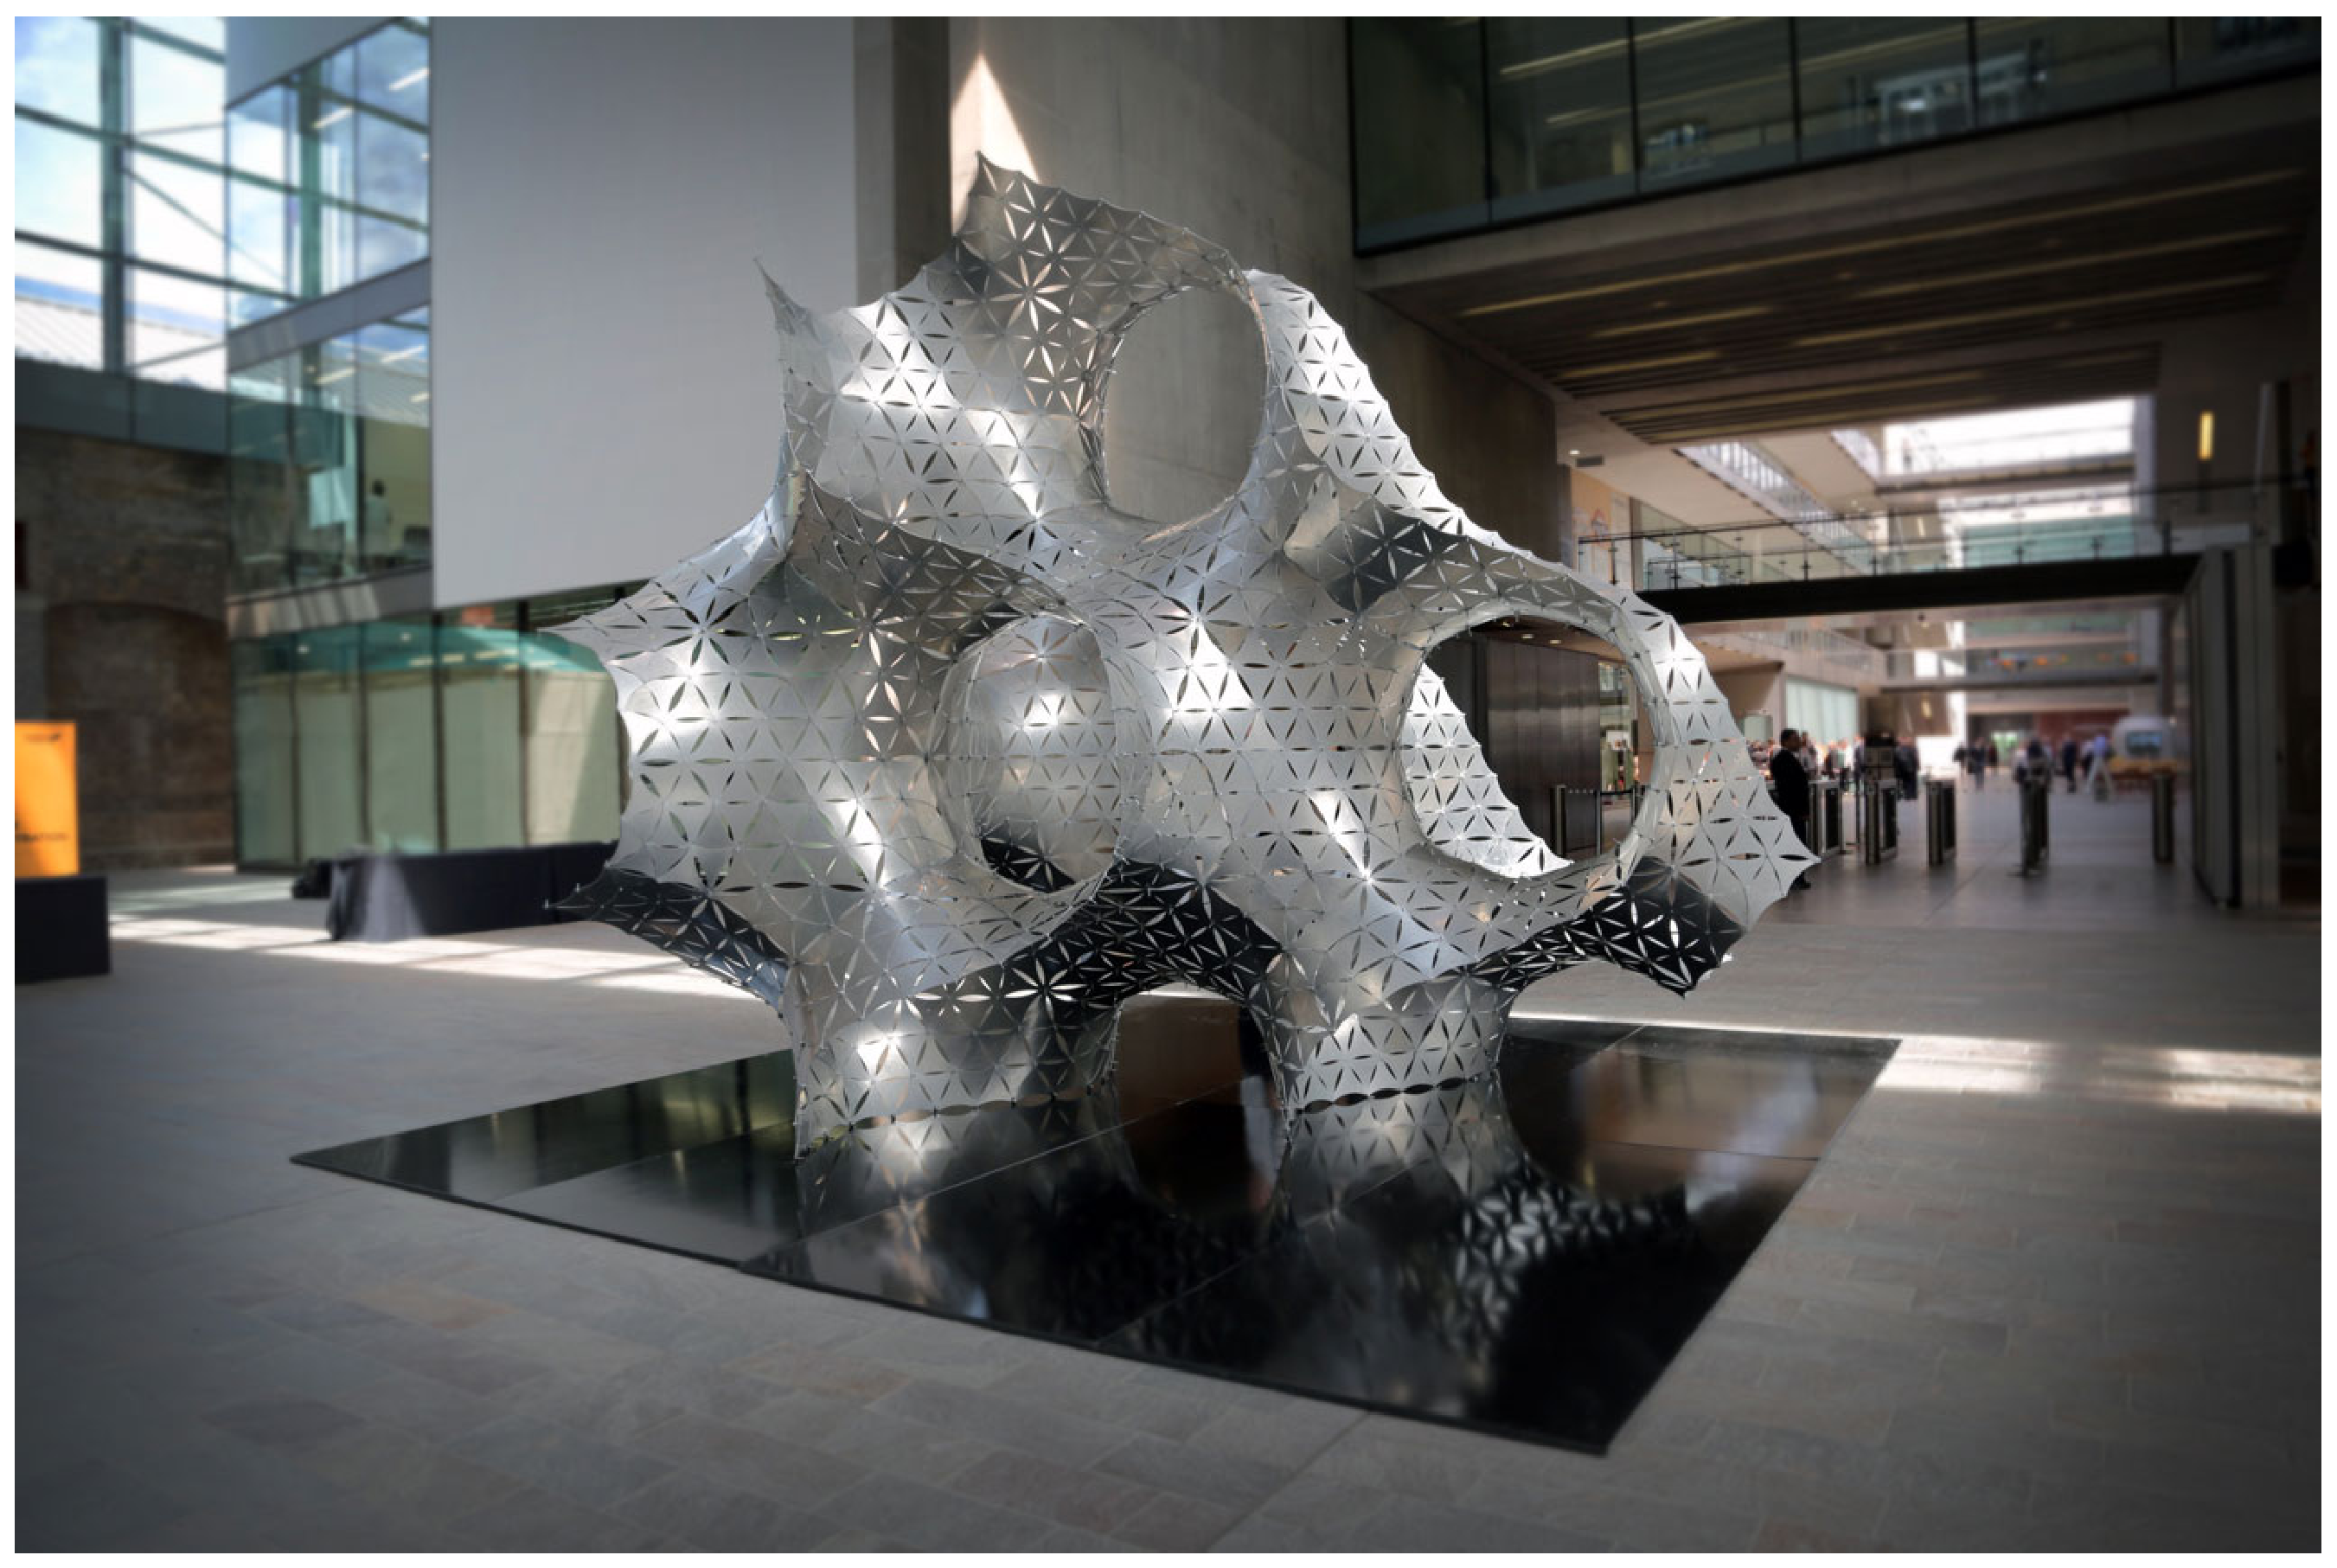
\includegraphics[scale=0.11]{musee.eps}
   \end{minipage}
    \begin{minipage}[b]{0.50\linewidth}   
     \centering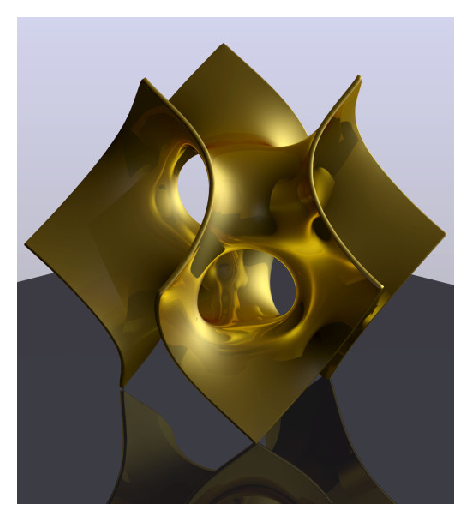
\includegraphics[scale=0.45]{goldenbatwing.eps}
   \end{minipage}
\end{figure}
\end {frame}
\section{Théorie}
\subsection{Surfaces}
\begin {frame}
\frametitle{Surfaces}
  $\mathscr{U}$ est une partie de $\R^2$.\\
  $\bullet$ Un \gs{patch} (ou surface locale, ou nappe) régulier est une application $x:\mathscr{U}\rightarrow \R^3$ différentiable, de matrice jacobienne de rang $2$.\\
  On confond l'application et son image $x(\mathscr{U})$ en général.\\
 \pause 
$\bullet$ Une \gs{surface} est composée d'un ou plusieurs patchs : en chaque point, il existe un voisinage qui est image d'un patch. 
\end {frame}

\begin {frame}
\frametitle{Sphère}
Une sphère par exemple n'est pas un patch régulier : \\ une paramétrisation est :\\
$x : \begin{array}[t]{ccccc}[0,2\pi] &\times& \left[-\frac{\pi}{2},\frac{\pi}{2}\right]&\rightarrow & \R^3\\
(u&,&v)&\rightarrow &(cos\ v\ cos\ u, cos\ v\ sin\ u, sin\ v)\\ \end{array}$\\
\pause
\vspace{1cm}
$$\mathscr{J}_x(u,v) = \left[\begin{array}{cc} 
-cos\ v\ sin\ u & -sin\ v\ cos\ u\\
cos\ v\ cos\ u & -sin\ v\ sin\ u \\ 
0 & cos\ v \\ \end{array}\right]$$
\pause
Donc pour le pôle nord $\left(v=\frac{\pi}{2}\right)$, la matrice jacobienne devient : \\
$\mathscr{J}_x\left(u,\frac{\pi}{2}\right) = \left[\begin{array}{cc} 
0 & -cos\ u\\
0 & -sin\ u \\ 
0 & 0 \\ \end{array}\right]$, qui est clairement de rang $1$.
\end {frame}

\begin {frame}
\frametitle{Sphère}
Mais une sphère est une surface, car peut être recouverte par deux patchs : 
\pause
\begin{figure}[h!]
      \centering 
      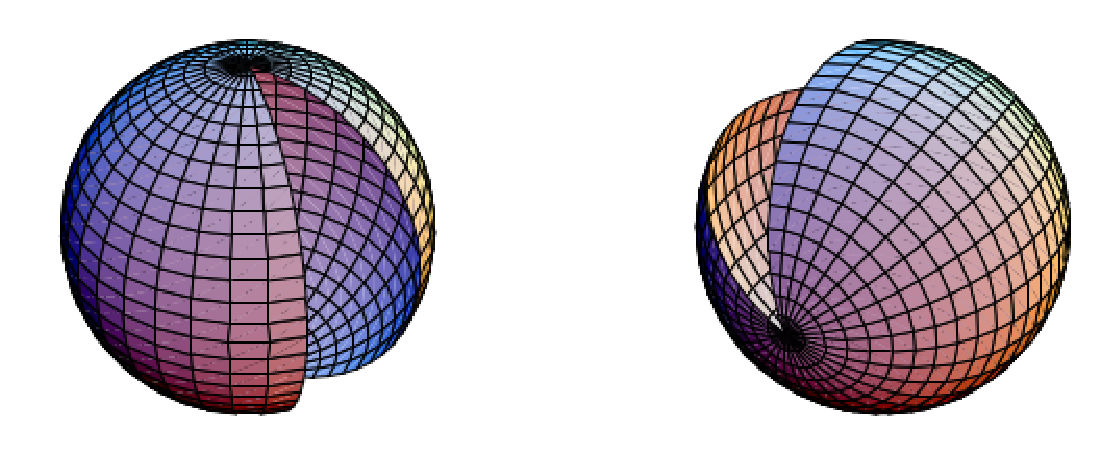
\includegraphics[scale=0.5]{1.eps}
      \legend{Deux patchs formant une sphère}
\end{figure}
\end {frame}

\subsection{Courbure d'une surface}

\begin {frame}
  \frametitle{Courbure}
  \begin{itemize}
  \item $p$ un point d'une surface $\mathscr{M}$
  \item $u_p$ vecteur unitaire tangent à $\mathscr{M}$ en $p$
  \item $U$ champ de vecteurs normal à $\mathscr{M}$\\
  \end{itemize}
\pause
On appelle \gs{courbure normale de $\mathscr{M}$ dans la direction $u_p$} le nombre réel
$$k(u_p)=(-D_{u_p}\cdot U)\cdot u_p, $$
\pause
$k(u_p)>0$ :  $\mathscr{M}$ se courbe dans la même direction que $U(p)$ \\
$k(u_p)<0$ :  $\mathscr{M}$ se courbe dans la direction opposée que $U(p)$ \\
$k(u_p)=0$ : $\mathscr{M}$ ne se courbe pas.
\end{frame}

\begin{frame}
\begin{figure}[h!]
      \centering 
      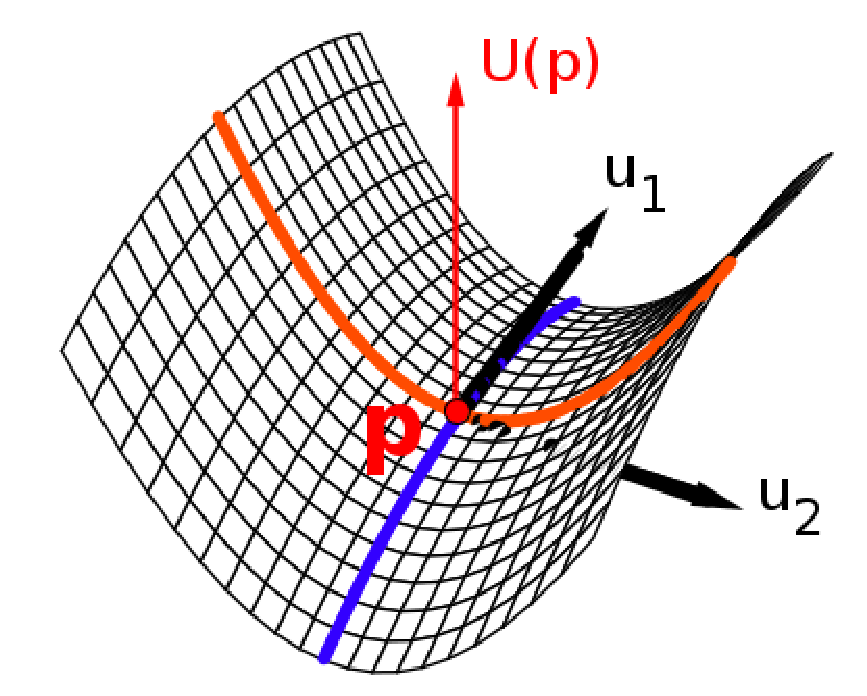
\includegraphics[scale=0.5]{2a.eps}
\end{figure} 
\pause
La surface a une courbure négative selon le vecteur $u_1$, et une positive selon le vecteur $u_2$ : 
\end {frame}

\subsection{Surface minimale}
\subsubsection{Courbures principales}

\begin{frame}
\frametitle{Courbure principale}
Les \gs{courbures principales} de $\mathscr{M}$ en $p$, notées $k_1$ et $k_2$, sont les maximum et minimum des courbures normales à $p$, $u_p$ parcourant l'ensemble des vecteurs unitaires tangents à $p$.\\
\begin{figure}[h!]
      \centering 
      \legend{}
      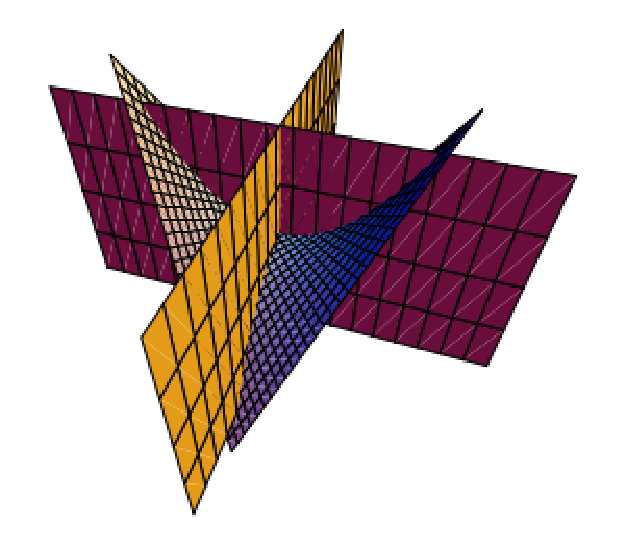
\includegraphics[scale=0.5]{2.eps}
\end{figure}
\end{frame}

\subsubsection{Définition}

\begin{frame}
\frametitle{Définition}
$\bullet$ $\frac{k_1+k_2}{2}$ est la \gs{courbure moyenne} de la surface en $p$.\vspace{0.5cm}\\
\pause
$\bullet$ Une \gs{surface minimale} est une surface pour laquelle en tout point la courbure moyenne vaut 0.\vspace{0.5cm}\\
\pause
D'après la définition d'une surface minimale, on a donc en chaque point d'une telle surface, la courbure maximale qui est égale à l'opposé de la courbure minimale.
\end{frame}

\subsubsection{Exemples}

\begin{frame}
\frametitle{Le caténoïde}
\gs{Exemples} : 
\pause \\
$\bullet$ Première surface minimale non plane, découverte en 1744 par Euler
\begin{figure}[h!]
      \centering 
      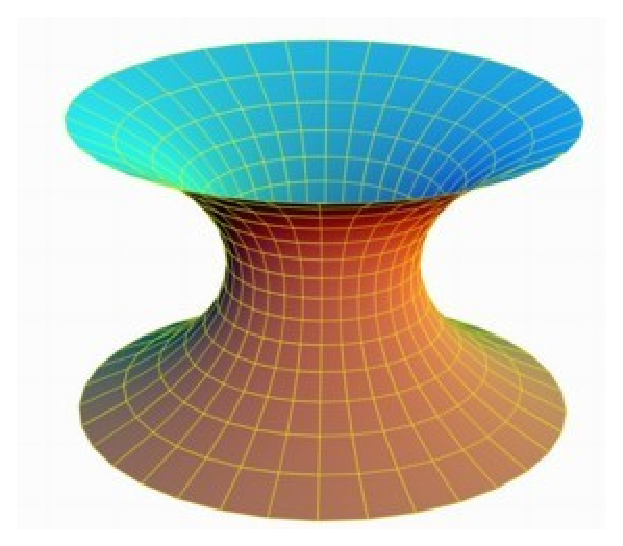
\includegraphics[scale=0.5]{3.eps}
      \legend{Un caténoïde}
\end{figure}
\end{frame}

\begin{frame}
\frametitle{L'hélicoïde}
$\bullet$ Découverte en 1776 par Meusnier
\begin{figure}[h!]
      \centering 
      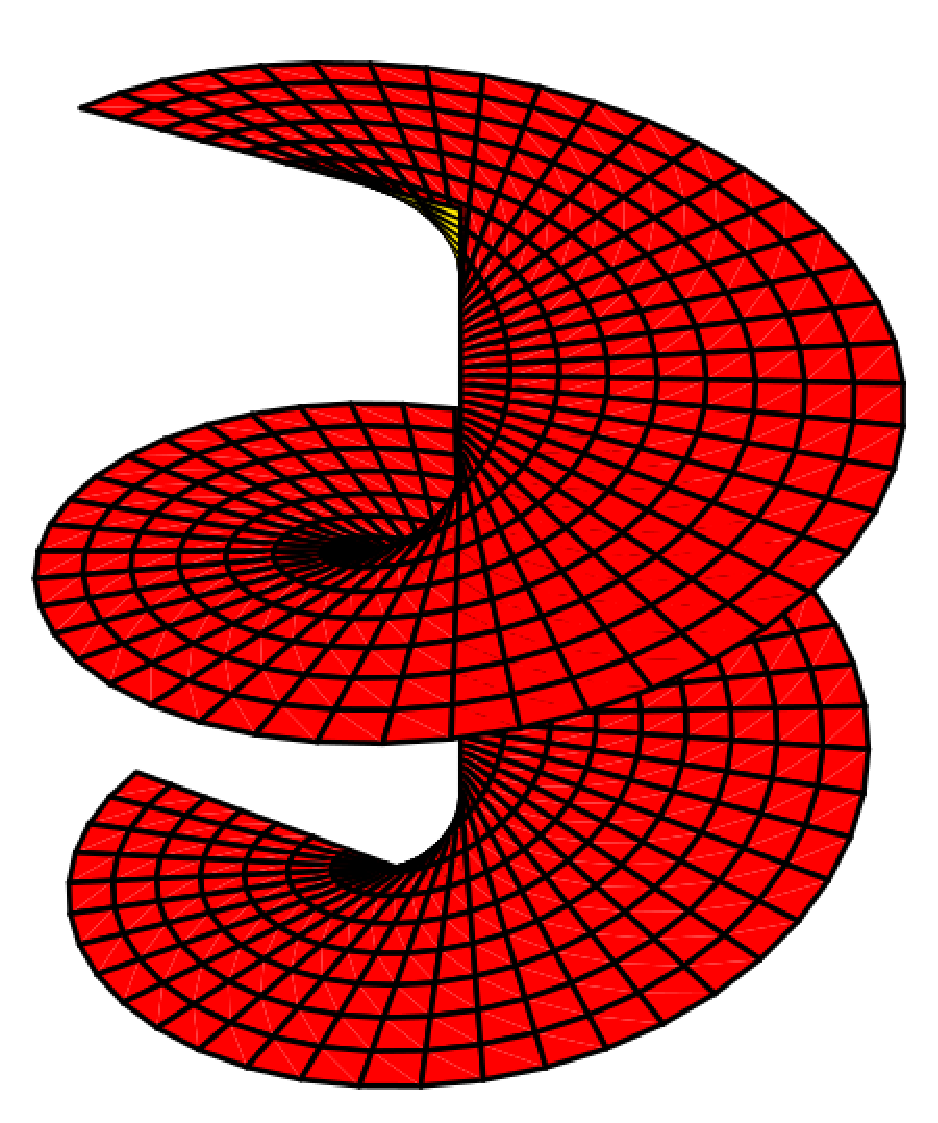
\includegraphics[scale=0.30]{4.eps}
      \legend{Un hélicoïde}
\end{figure}
\end{frame}

\begin{frame}
\frametitle{La surface d'Enneper}
$\bullet$ Découverte en 1863 par Enneper\\
$\bullet$ A des auto-intersections
\begin{figure}[h!]
      \centering 
      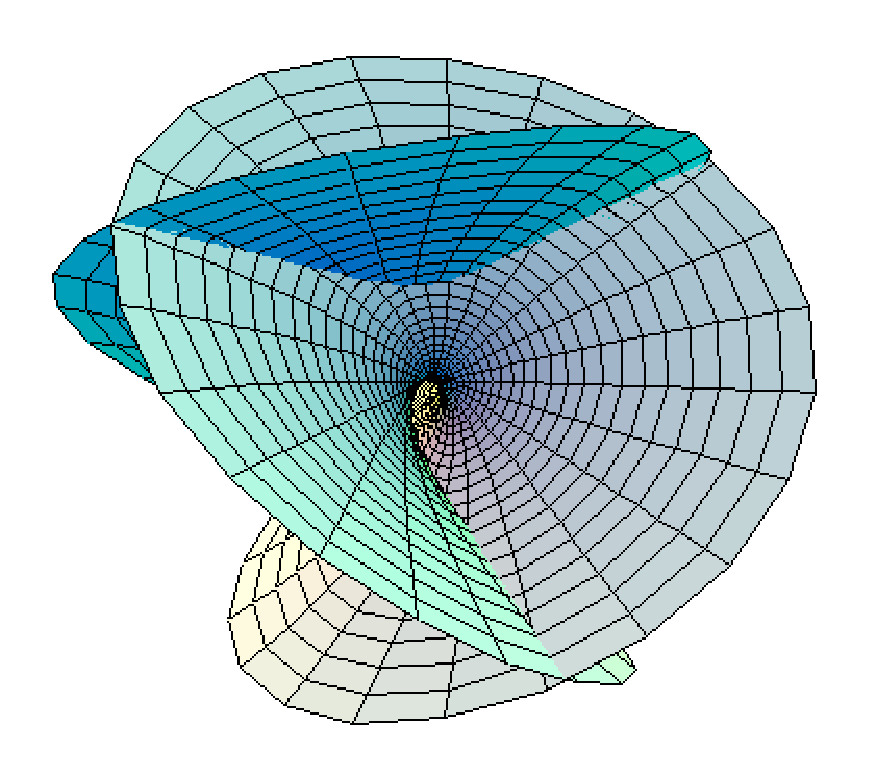
\includegraphics[scale=0.42]{5.eps}
      \legend{Surface d'Enneper}
\end{figure}
\end{frame}

\begin{frame}
\frametitle{Familles de surfaces minimales - Exemple}
\begin{center}
\animategraphics[autoplay,loop,scale = 0.3]{2}{HelicoideDeformee/helicoideDeformee-}{0}{6} 
\end{center}
\end{frame}

\subsubsection{Pourquoi minimale ?}

\begin{frame}
\frametitle{Pourquoi minimale ?}
Une surface minimale a aussi une aire minimale parmi toutes les surfaces "légèrement déformées" ayant le même bord. \\
\pause
Plus précisément, soit $x$ un patch, $U$ un champ de vecteurs normaux, et $h:\mathscr{U}\rightarrow \R$ :\\
$\bullet$ Une déformation normale de $x$ est une application : 
$$X:]-\epsilon , \epsilon[\times \mathscr{U} \rightarrow \R^3\text{, avec } \epsilon >0 \text{ et } $$ 
$$ X(t, p) = x(p)+\underbrace{t\cdot h(p)}_{\in \R}\cdot U(p)$$
\pause
$t\mapsto X(t, \cdot)$ représente donc une déformation continue de la surface $x$, chaque point étant éloigné perpendiculairement de cette surface.
\end{frame}

\begin{frame}
\frametitle{Théorème}
\gs{Théorème} : $x$ est minimale sur $\mathscr{U}$ ssi $\forall h:\mathscr{U} \rightarrow \R,$ $$ A'(x)=0.$$
$A:\{X(t, \cdot)\}\rightarrow \R$ est la fonction qui donne l'aire.\\
\pause
\vspace{1cm}
$\bullet$ On a donc un minimum local.\\
\end{frame}

\begin{frame}
Attention, surface minimale $\nRightarrow$ aire minimale : \\
\begin{figure}[h!]
      \centering 
      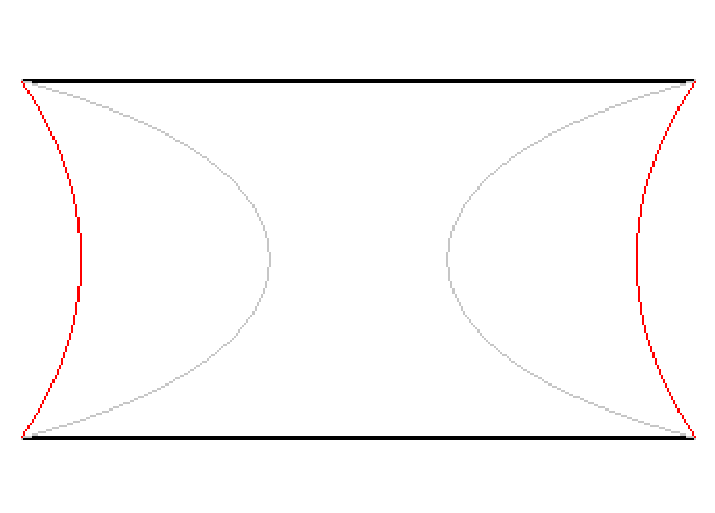
\includegraphics[scale=0.37]{3a.eps}
      \legend{Trois surfaces minimales}
\end{figure}
$\bullet$ Trois surfaces minimales : \\un caténoïde (en rouge), un "pseudo-caténoïde" (en gris), et la surface de Goldbach (deux disques dans les cercles).\\
\pause
Tout dépend de l'écartement des cercles : \\
$\bullet$ proches : le caténoïde rouge est d'aire minimale\\
$\bullet$ écartés : la surface de Goldbach est d'aire minimale\\
\end{frame}

\section{Problème de Plateau}
\subsection{Exposé}
\begin{frame}
\frametitle{Problème de Plateau} 
$\bullet$ Problème posé par Lagrange en 1760, mais qui porte le nom de Plateau qui étudia des bulles de savon\\
\pause
$\bullet$ Existence de surfaces minimales, un bord étant donné (courbes fermées)\\
\pause
$\bullet$ Résolution en 1931 (Douglas) $\Rightarrow$ médaille Fields :\\
\pause
\begin{itemize}
\item Il y a toujours au moins une surface minimale\\
\item Il y en a un nombre fini\\
\item Une seule est d'aire minimale et elle ne présente pas d'auto-intersection\\
\end{itemize}
\pause
\gs{Problème} : Comment les construire ?\\
En particulier si les courbes de départ sont compliquées...\\
\end{frame}


\subsection{Algorithme}
\begin{frame}
\frametitle{Algorithme}
$\Longrightarrow$ algorithme itératif\\
$\bullet$ \gs{Entrée} : une surface de départ représentée par un maillage triangulaire et un ensemble de points (les bords)\\
$\bullet$ \gs{Sortie} : une surface très proche d'une surface minimale\\
L'algorithme va déformer petit à petit la surface de départ pour se rapprocher d'une surface minimale
\end{frame}

\begin{frame}
\frametitle{Algorithme}
Entre deux itérations, on modifie chaque point du maillage avec une fonction $f$.\\
Si $E(f)$, l'énergie de $f$, est minimale, la surface obtenue est minimale :
$$E(f) = \frac{1}{2} \int_\mathscr{U} |\nabla f|^2 \text{ avec } |\nabla f|^2 = tr(^t\partial f \cdot \partial f).$$
L'idée est donc de rendre $E(f)$ de plus en plus petit au fur et à mesure de l'algorithme. \\
\end{frame}

\begin{frame}
\frametitle{Algorithme}
Un théorème dit que pour $f$ transformant un triangle $\Delta_1$ en $\Delta_2$, $$E(f) = \frac{1}{4}\sum_{i=1}^{3}cot\ \alpha_i\cdot |a_i|^2,$$ où :\\
$\bullet\ \alpha_i$ sont les angles du triangle $\Delta_1$\\
$\bullet$ $a_i$ est l'image dans $\Delta_2$ du côté opposé à $\alpha_i$.\\
\pause
En sommant sur tous les triangles de la surface, on obtient la formule cherchée : 
\end{frame}

\begin{frame}
\frametitle{Algorithme}
$$E(f) = \frac{1}{4}\sum_{i=1}^{\#bords} (cot\ \alpha_i + cot\ \beta_i) |a_i|^2.$$
\begin{figure}[h!]
      \centering 
      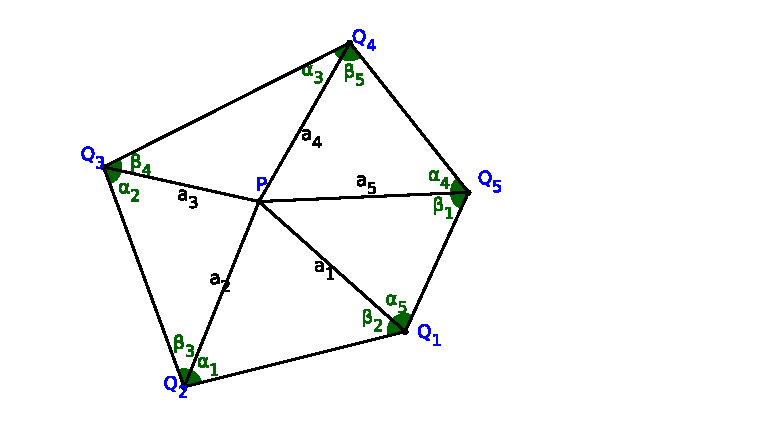
\includegraphics[scale=0.8]{6.eps}
\end{figure}
\end{frame}

\begin{frame}
\frametitle{Algorithme}
$\frac{\partial}{\partial p}E(f) = 0 \Longleftrightarrow$ \\
$$\frac{1}{2}\sum_{i=1}^{\#\text{voisins de }p} (cot\ \alpha_i + cot\ \beta_i) (p-q_i) = 0$$\pause
Ce qui donne, en isolant $p$ : \\
$$\boxed{p=\frac{\sum_{i=1}^{\#\text{voisins de }p}(cot\ \alpha_i + cot\ \beta_i) q_i}{\sum_{i=1}^{\#\text{voisins de }p}cot\ \alpha_i + cot\ \beta_i}}$$
Si tous les points $p$ de la surface vérifient cette formule, alors la surface est minimale.\\ \pause L'algorithme consiste donc à remplacer tous les points $p$ par le point vérifiant la formule ci-dessus, et à continuer.
\end{frame}

\subsection{Résultats}
\subsubsection{Caténoïde}

\begin{frame}
\frametitle{Caténoïde}
$\bullet$ Figure de départ : cylindre
\begin{figure}[h!]
      \centering 
      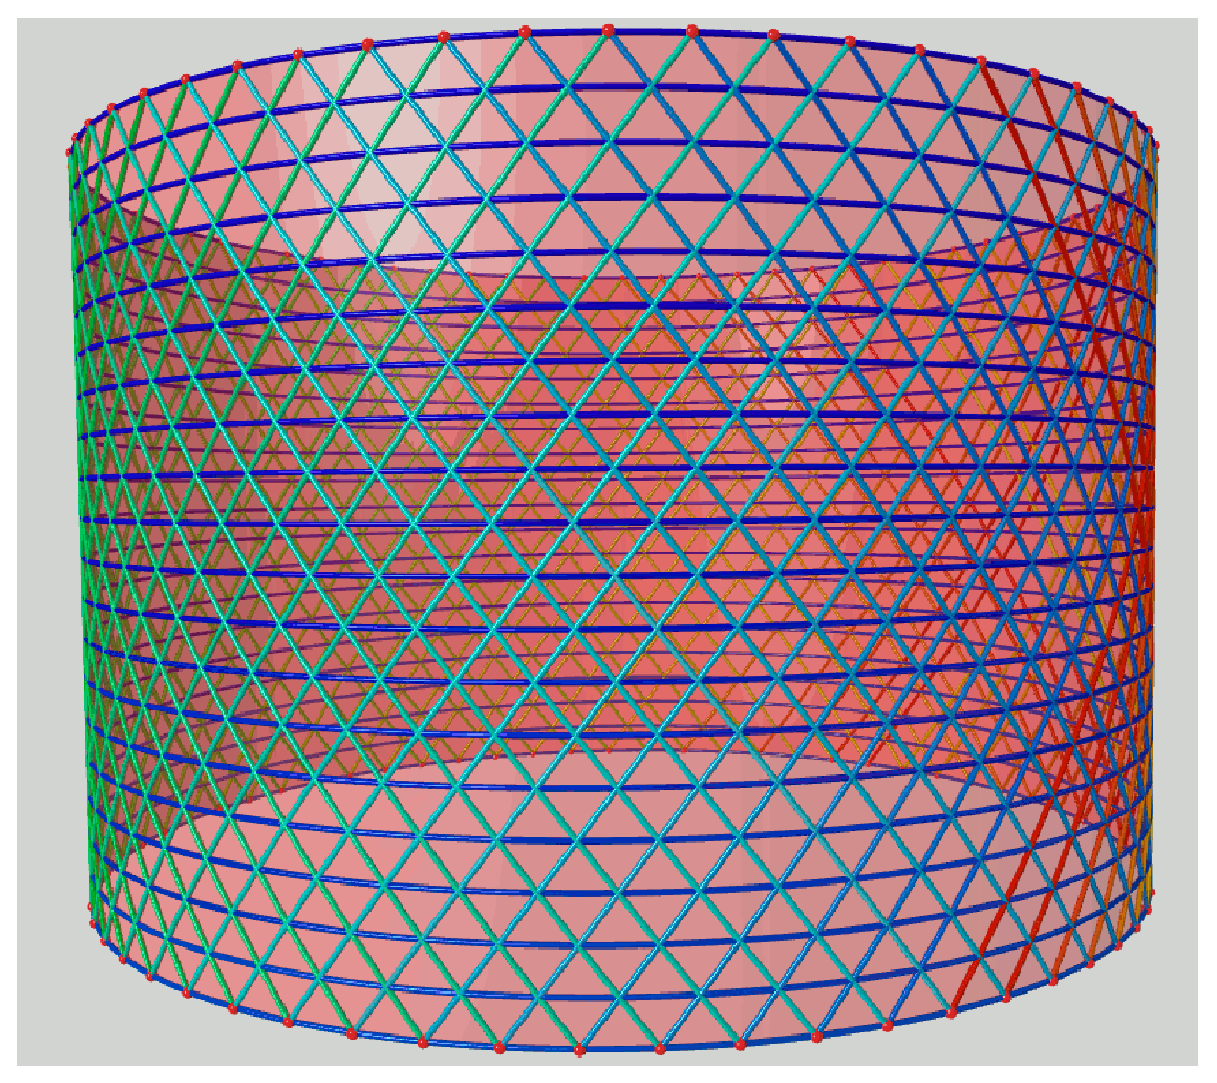
\includegraphics[scale=0.31]{catenoide/catenoide-0.eps}
\end{figure}
\end{frame}

\begin{frame}
\frametitle{Caténoïde}
\transduration{0.5}
Au fur et à mesure des itérations
\begin{figure}[h!]
      \centering 
      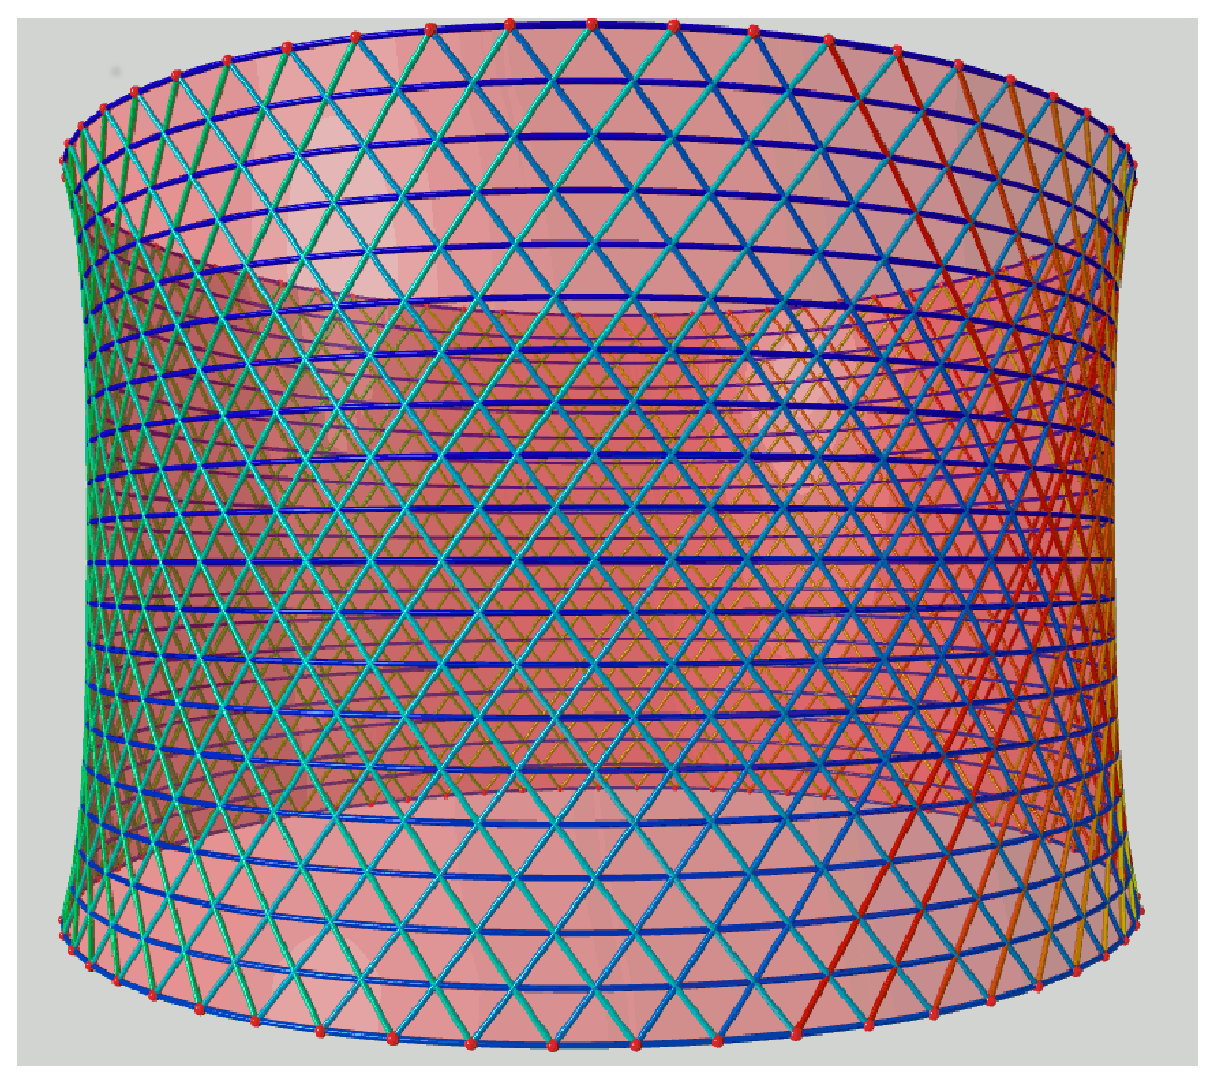
\includegraphics[scale=0.31]{catenoide/catenoide-1.eps}
\end{figure}
\end{frame}

\begin{frame}
\frametitle{Caténoïde}
\transduration{0.5}
Au fur et à mesure des itérations
\begin{figure}[h!]
      \centering 
      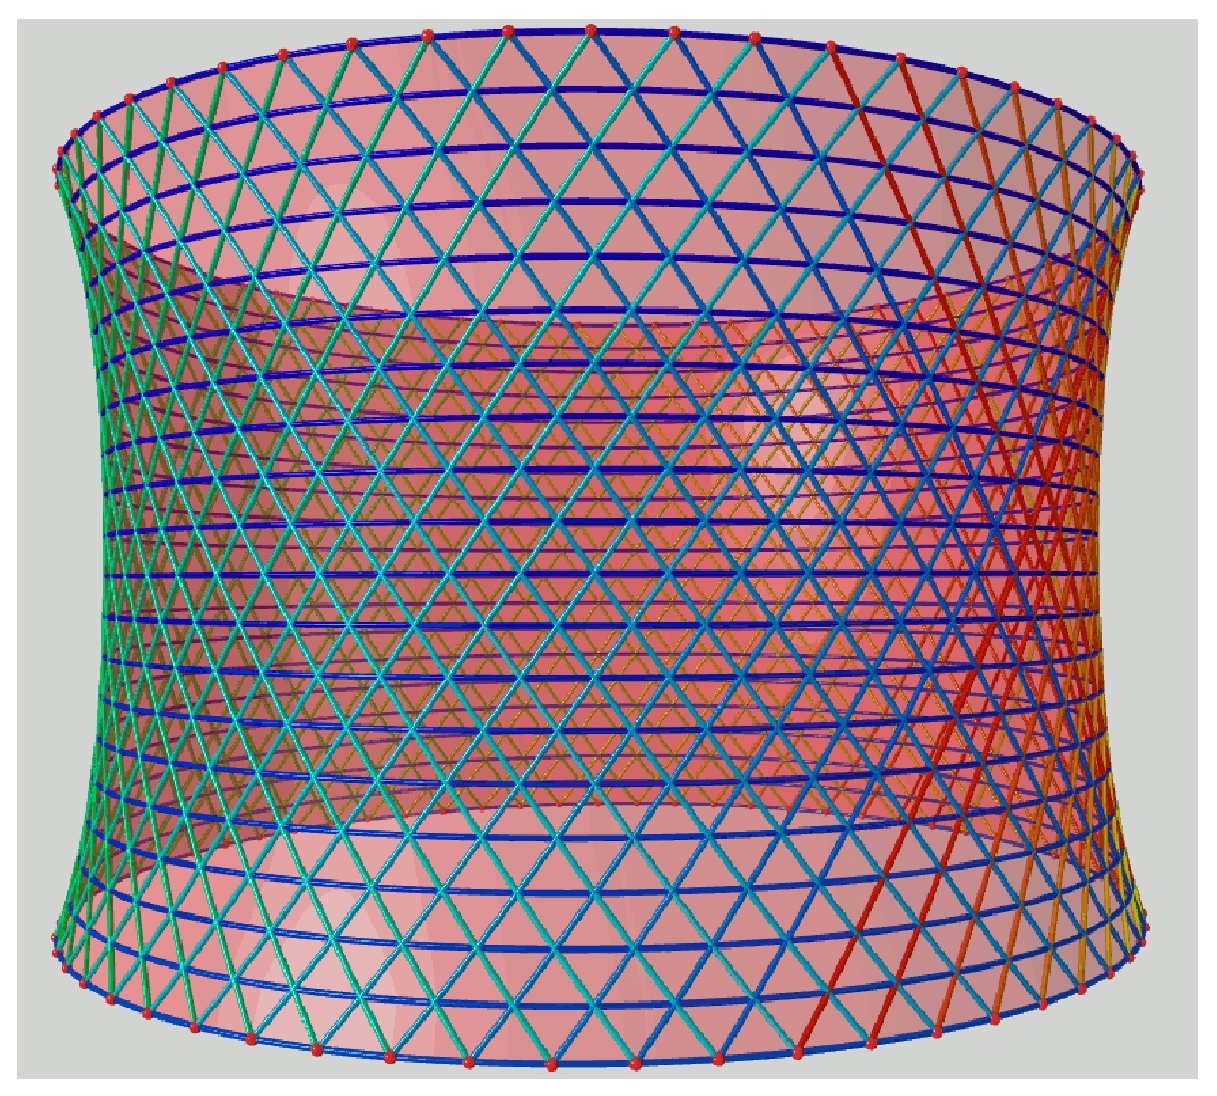
\includegraphics[scale=0.31]{catenoide/catenoide-2.eps}
\end{figure}
\end{frame}

\begin{frame}
\frametitle{Caténoïde}
\transduration{0.5}
Au fur et à mesure des itérations
\begin{figure}[h!]
      \centering 
      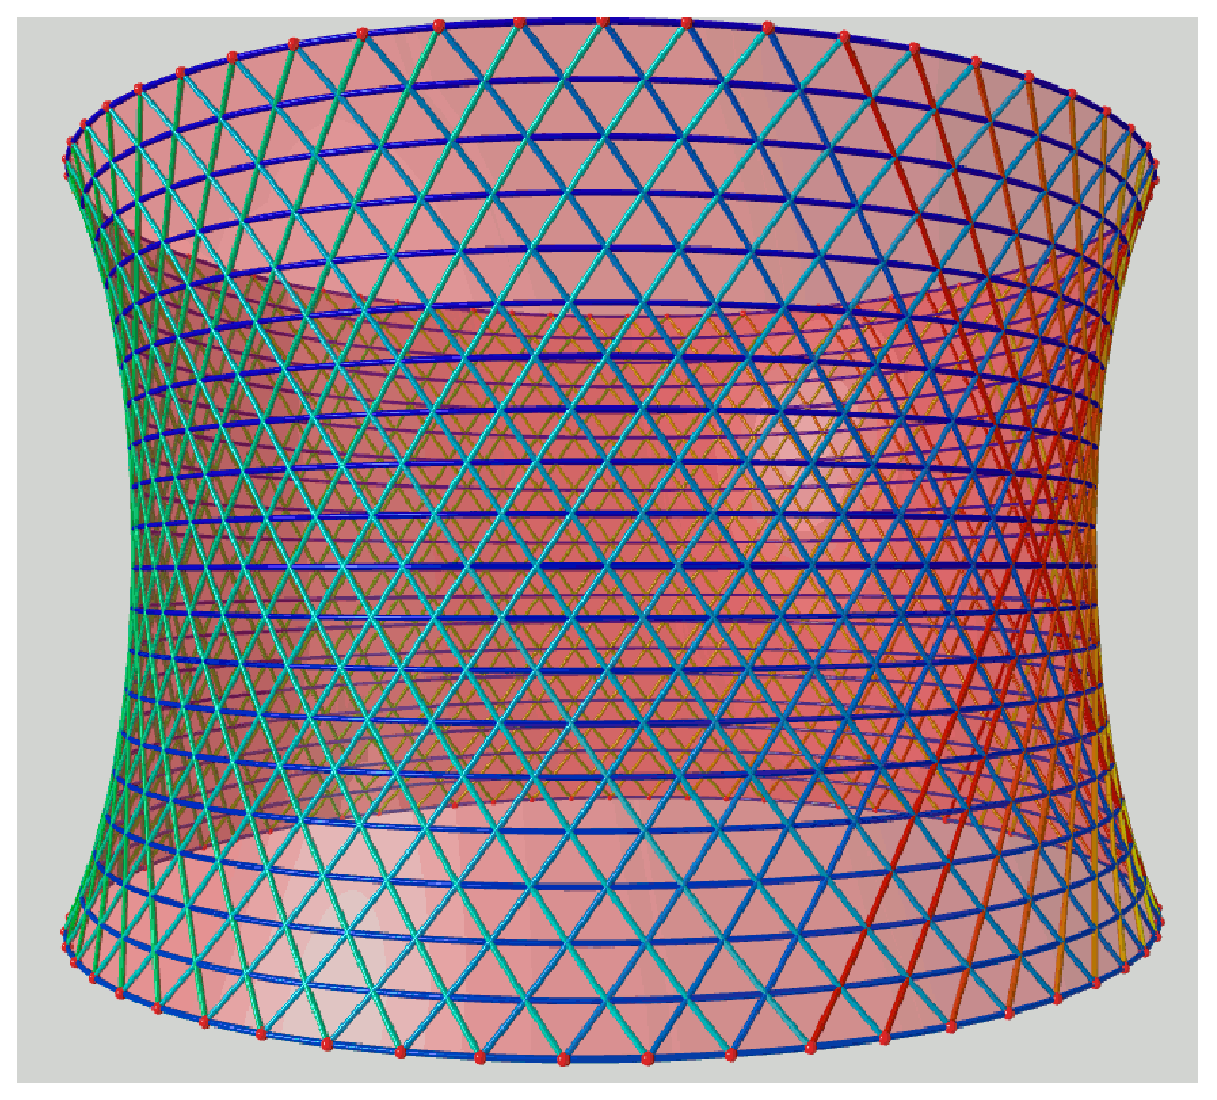
\includegraphics[scale=0.31]{catenoide/catenoide-3.eps}
\end{figure}
\end{frame}

\begin{frame}
\frametitle{Caténoïde}
\transduration{0.5}
Au fur et à mesure des itérations
\begin{figure}[h!]
      \centering 
      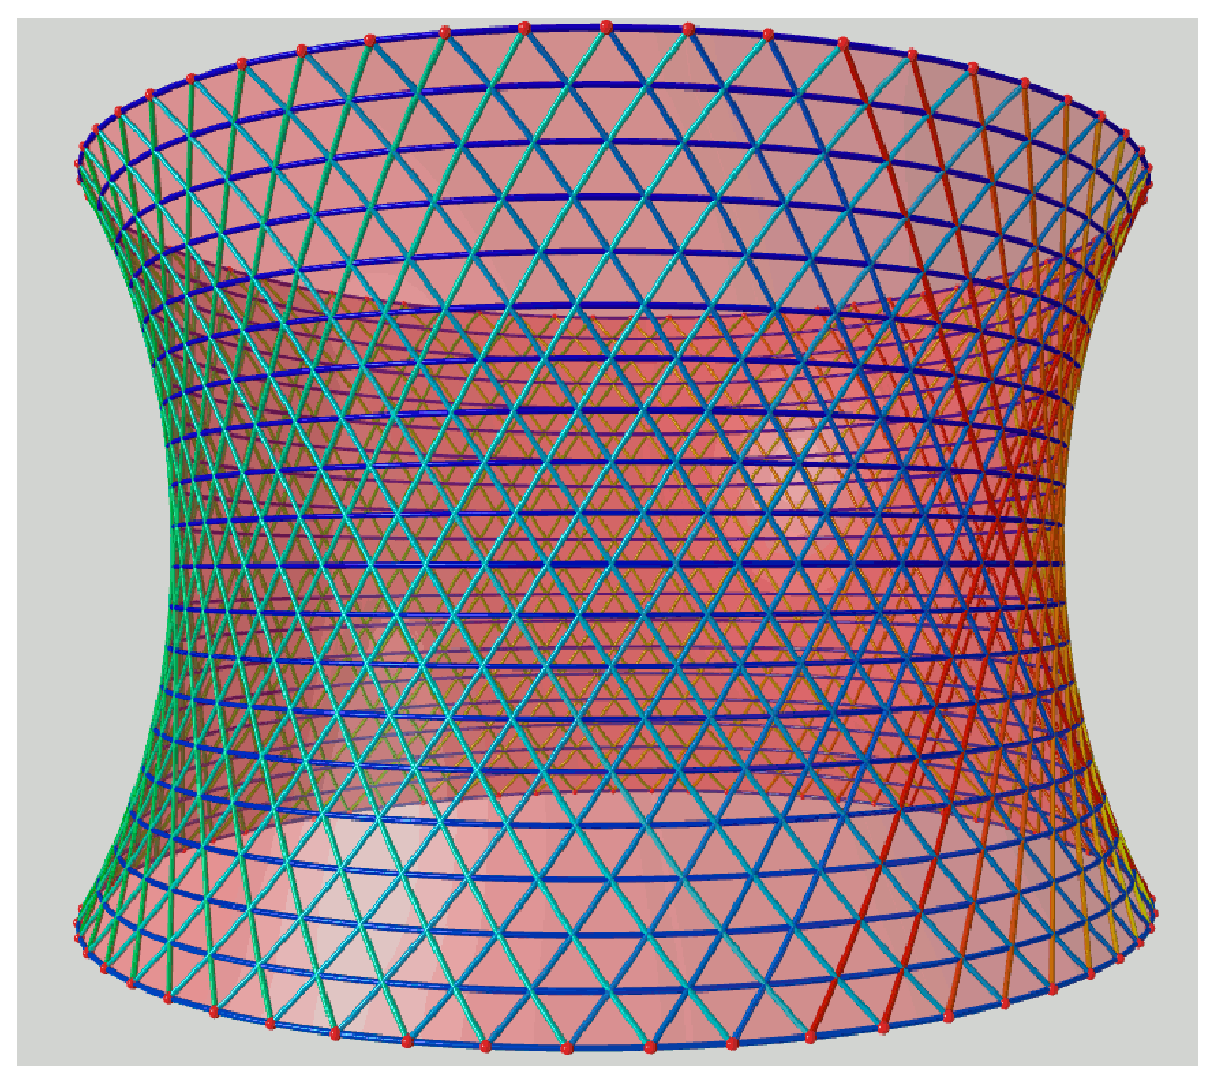
\includegraphics[scale=0.31]{catenoide/catenoide-4.eps}
\end{figure}
\end{frame}

\begin{frame}
\frametitle{Caténoïde}
\transduration{0.5}
Au fur et à mesure des itérations
\begin{figure}[h!]
      \centering 
      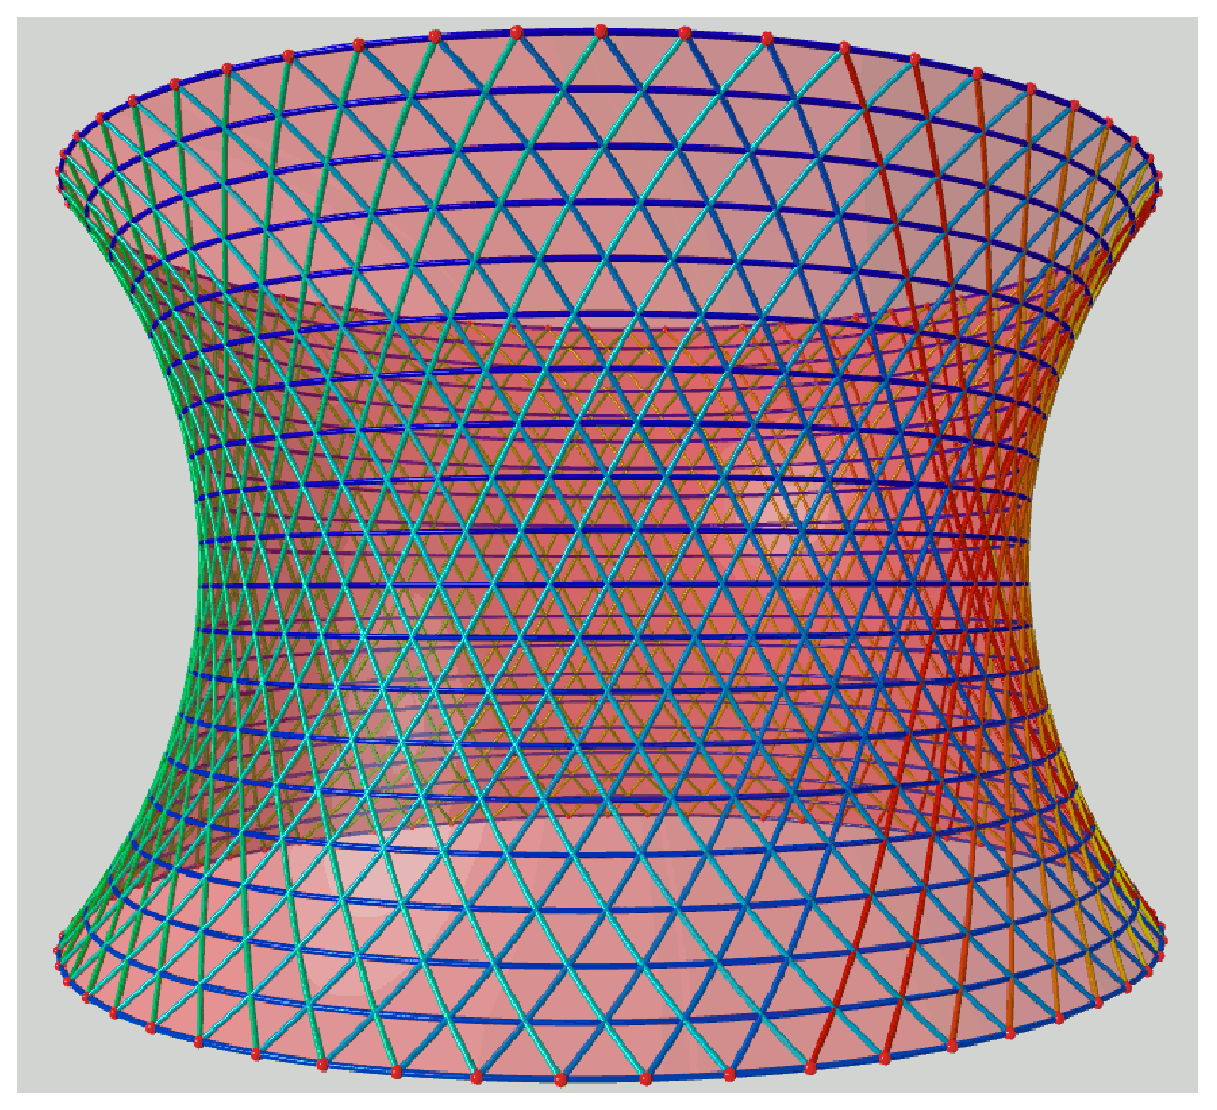
\includegraphics[scale=0.31]{catenoide/catenoide-5.eps}
\end{figure}
\end{frame}

\begin{frame}
\frametitle{Caténoïde}
\transduration{0.5}
Au fur et à mesure des itérations
\begin{figure}[h!]
      \centering 
      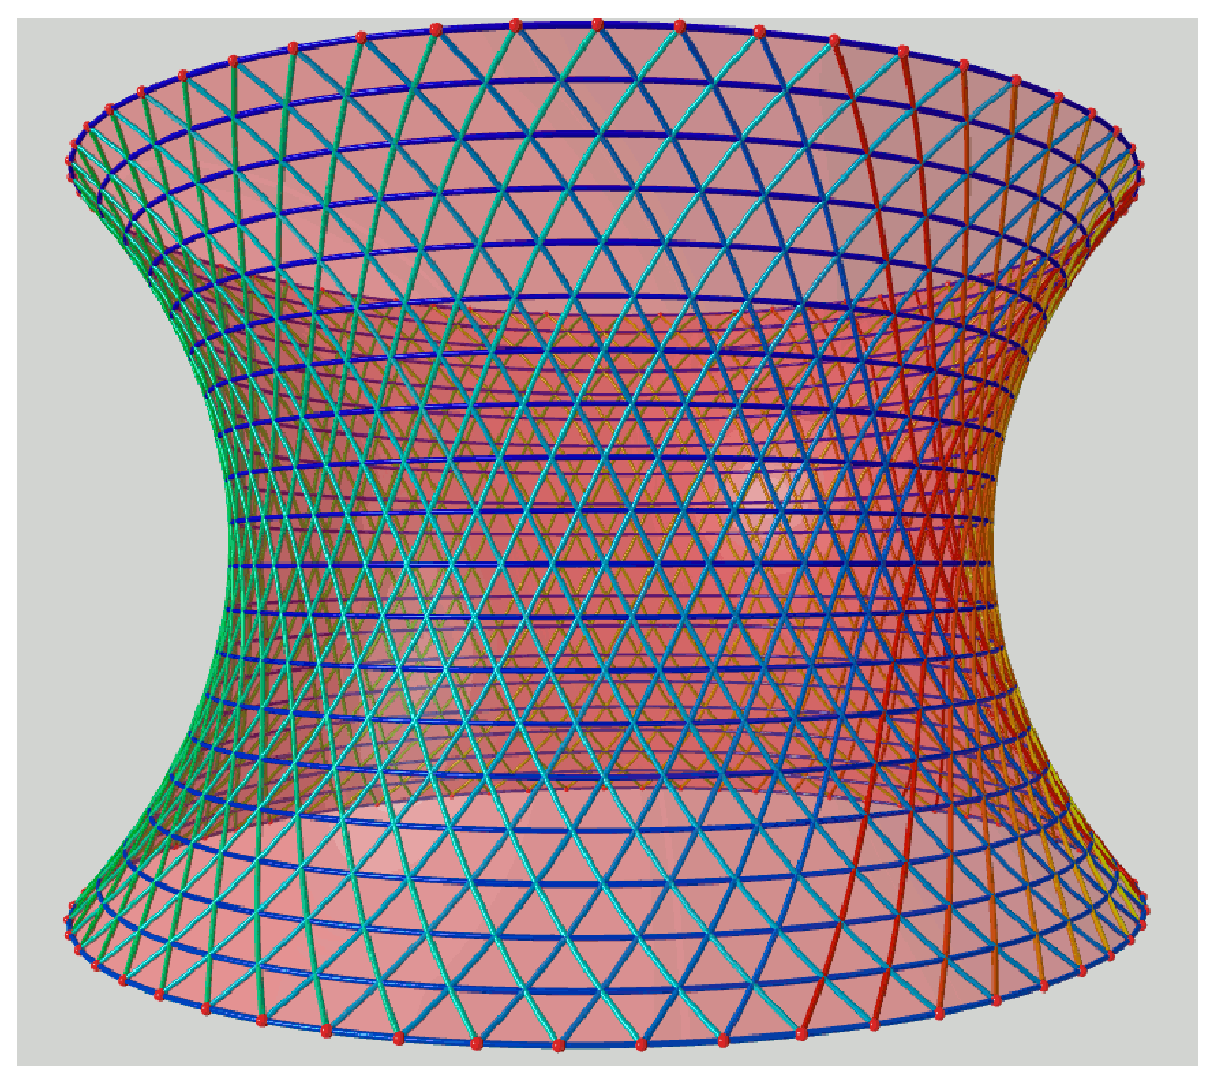
\includegraphics[scale=0.31]{catenoide/catenoide-6.eps}
\end{figure}
\end{frame}

\begin{frame}
\frametitle{Caténoïde}
\transduration{0.5}
Au fur et à mesure des itérations
\begin{figure}[h!]
      \centering 
      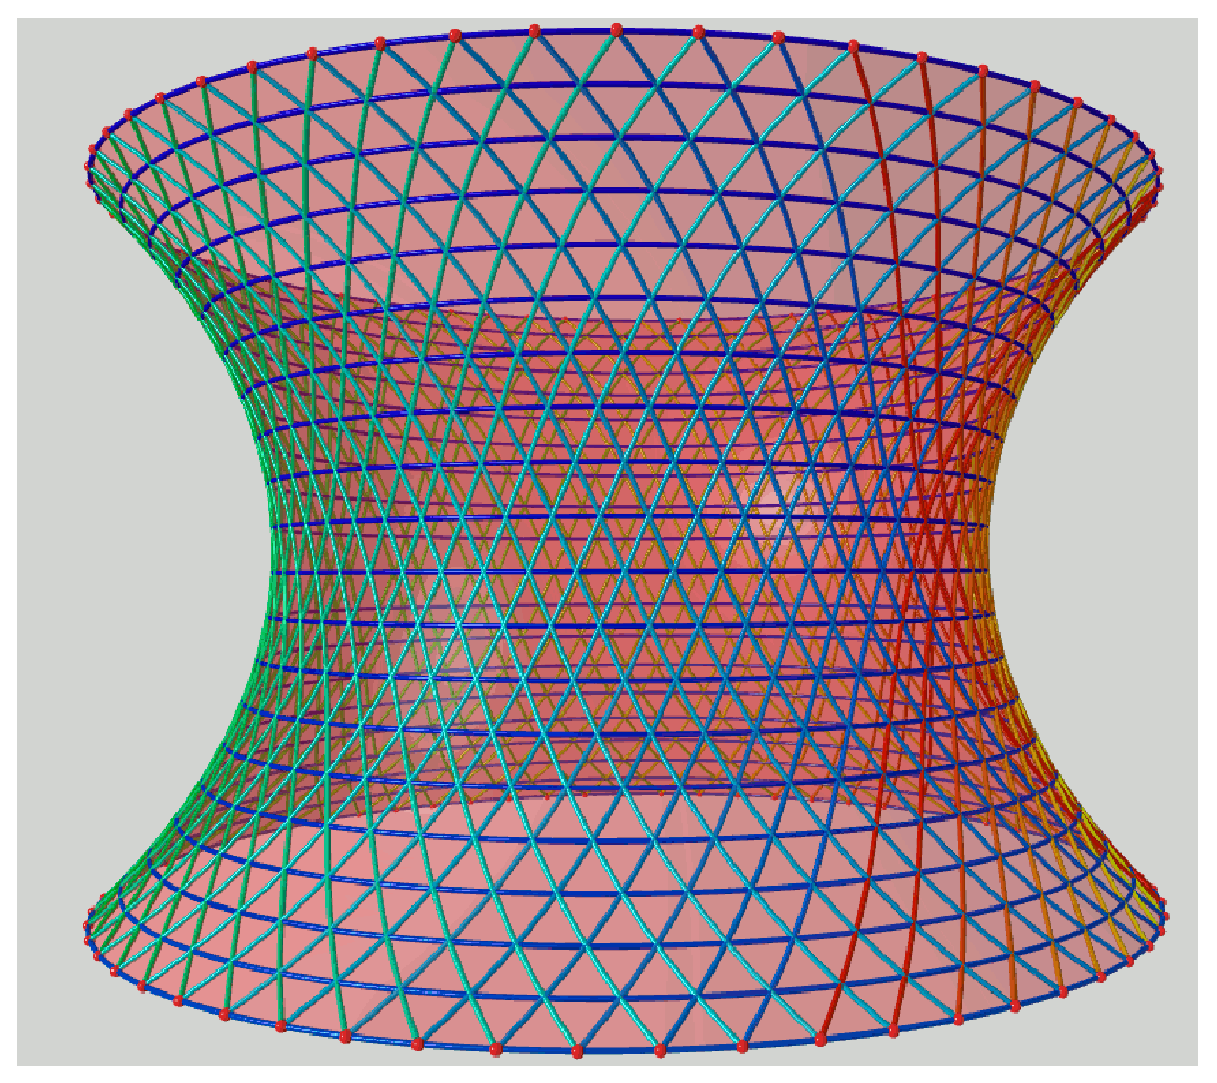
\includegraphics[scale=0.31]{catenoide/catenoide-7.eps}
\end{figure}
\end{frame}

\begin{frame}
\frametitle{Caténoïde}
\transduration{0.5}
Au fur et à mesure des itérations
\begin{figure}[h!]
      \centering 
      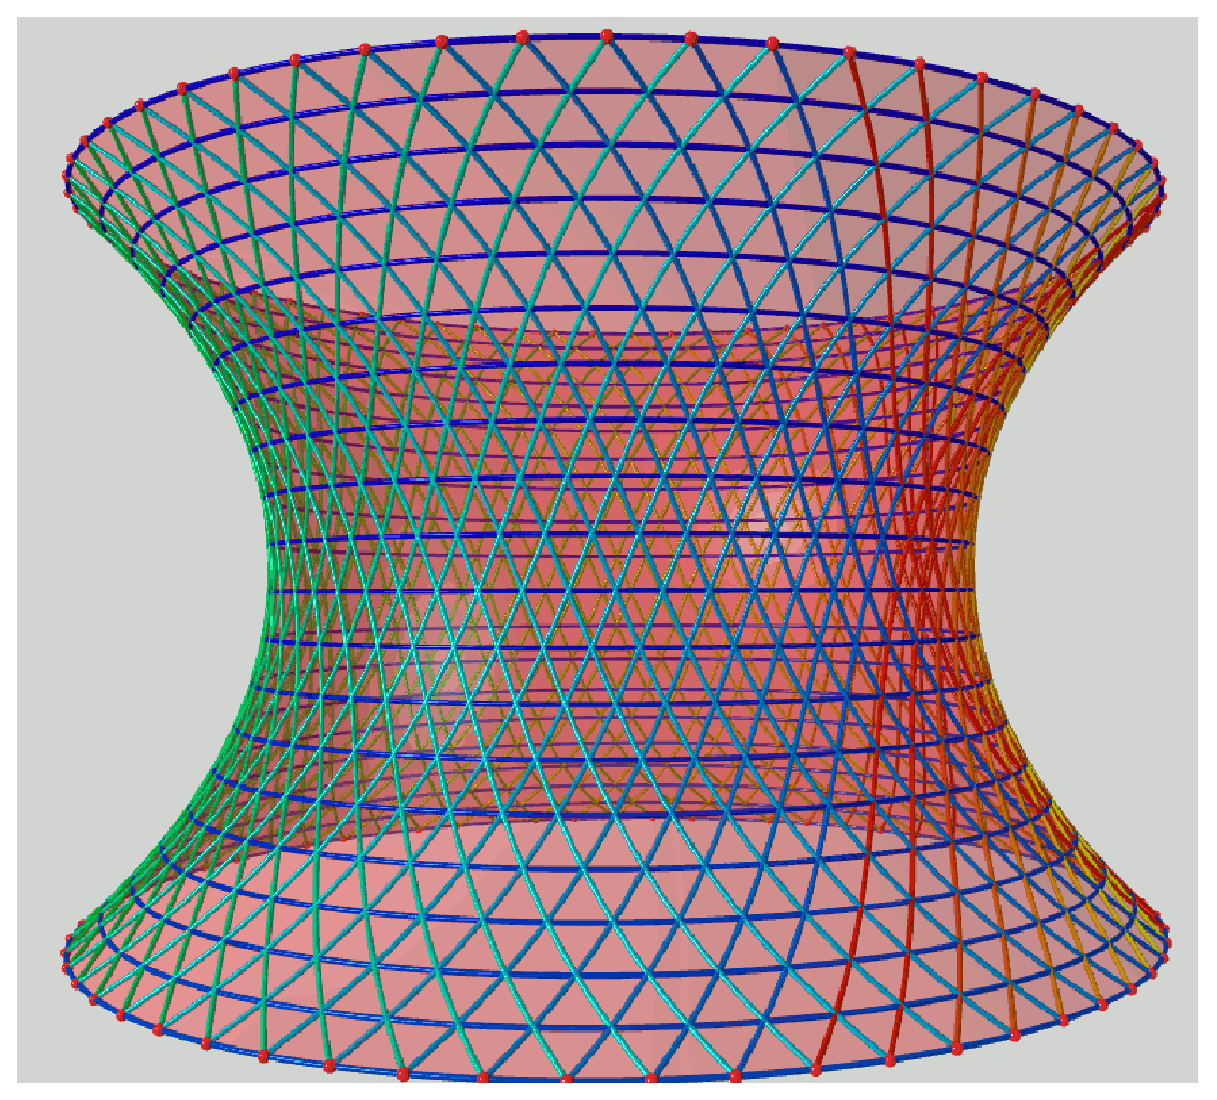
\includegraphics[scale=0.31]{catenoide/catenoide-8.eps}
\end{figure}
\end{frame}

\begin{frame}
\frametitle{Caténoïde}
Pour 1000 itérations : \\
\begin{figure}[h!]
      \centering 
      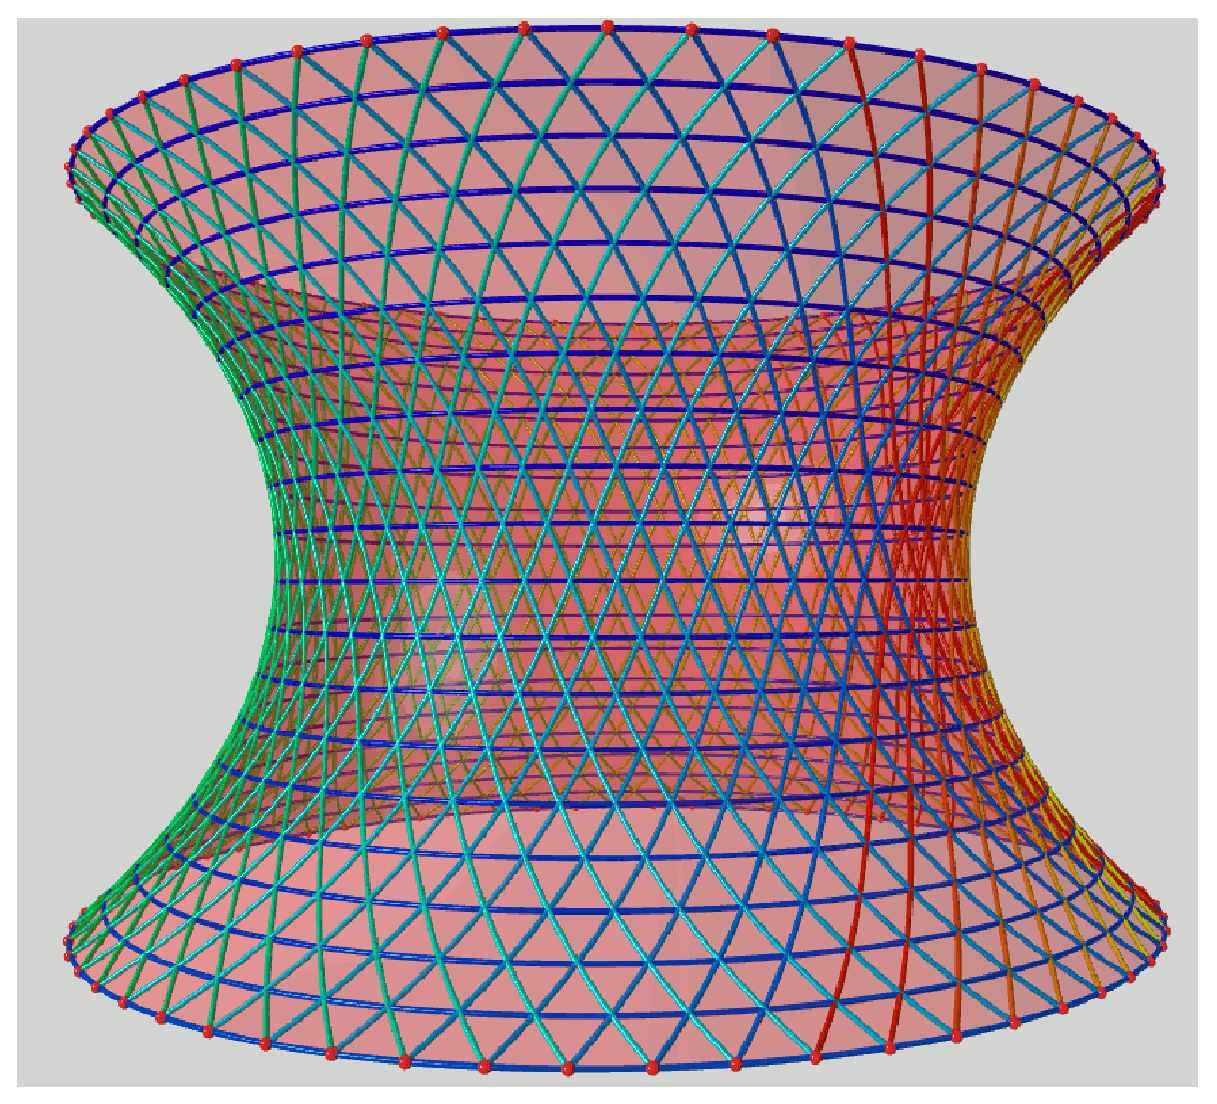
\includegraphics[scale=0.31]{catenoide/catenoide-9.eps}
\end{figure}
\end{frame}

\begin{frame}
\frametitle{Caténoïde - Cas limite}
\pause
\only<2>{
\begin{figure}[h!]
      \centering 
      \legend{200 itérations}
      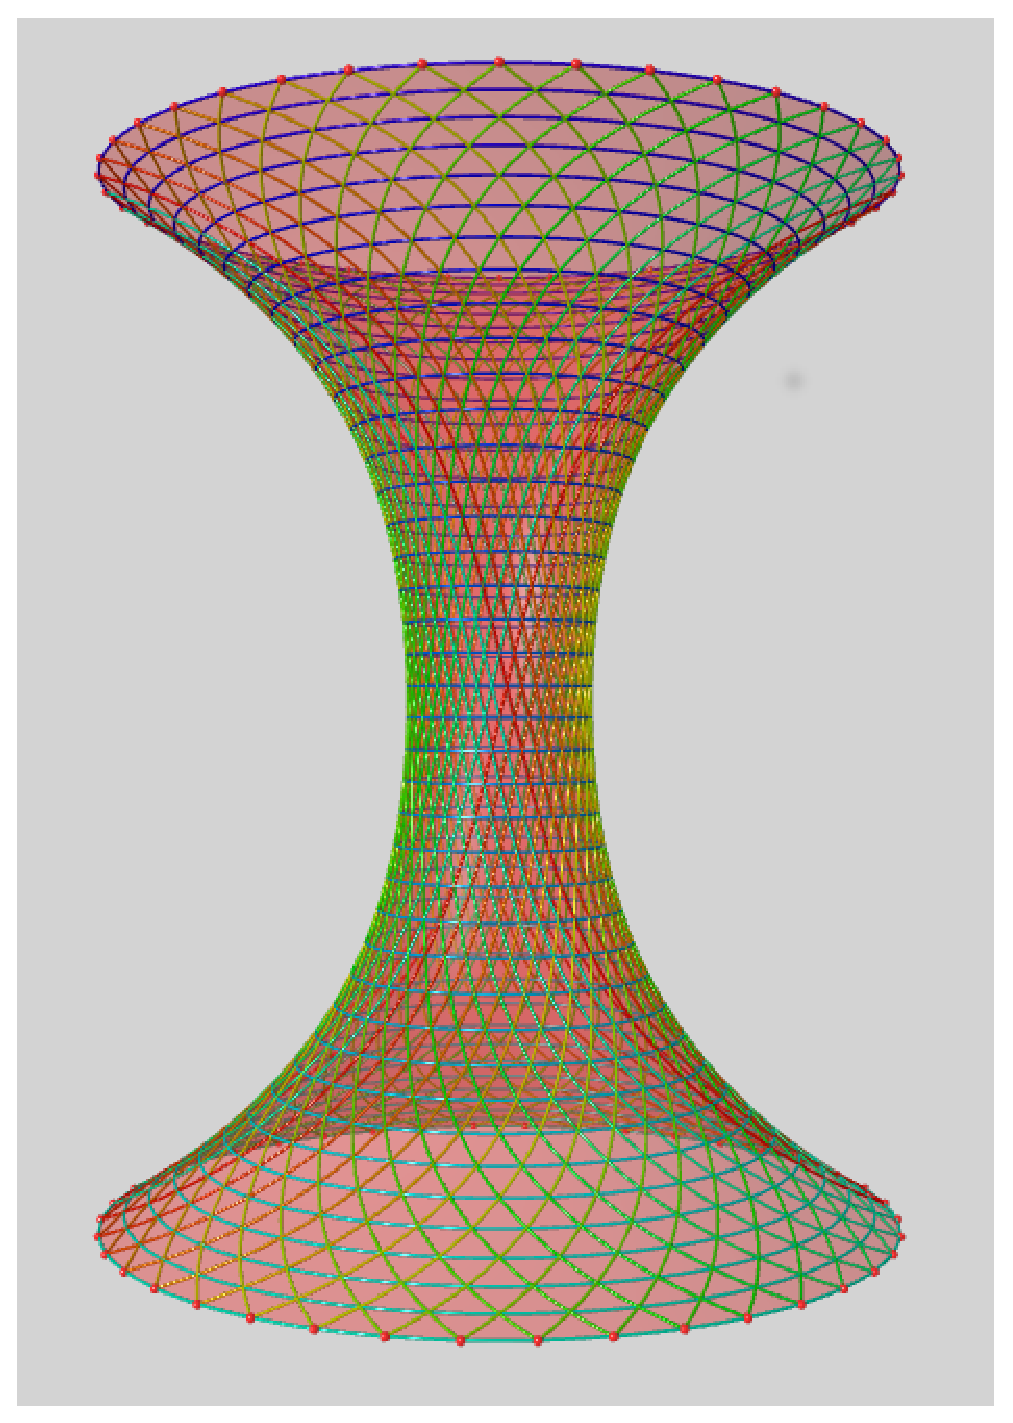
\includegraphics[scale=0.25]{7.eps}
\end{figure}
}
\only<3>{
\begin{figure}[h!]
      \centering 
      \legend{500 itérations}
      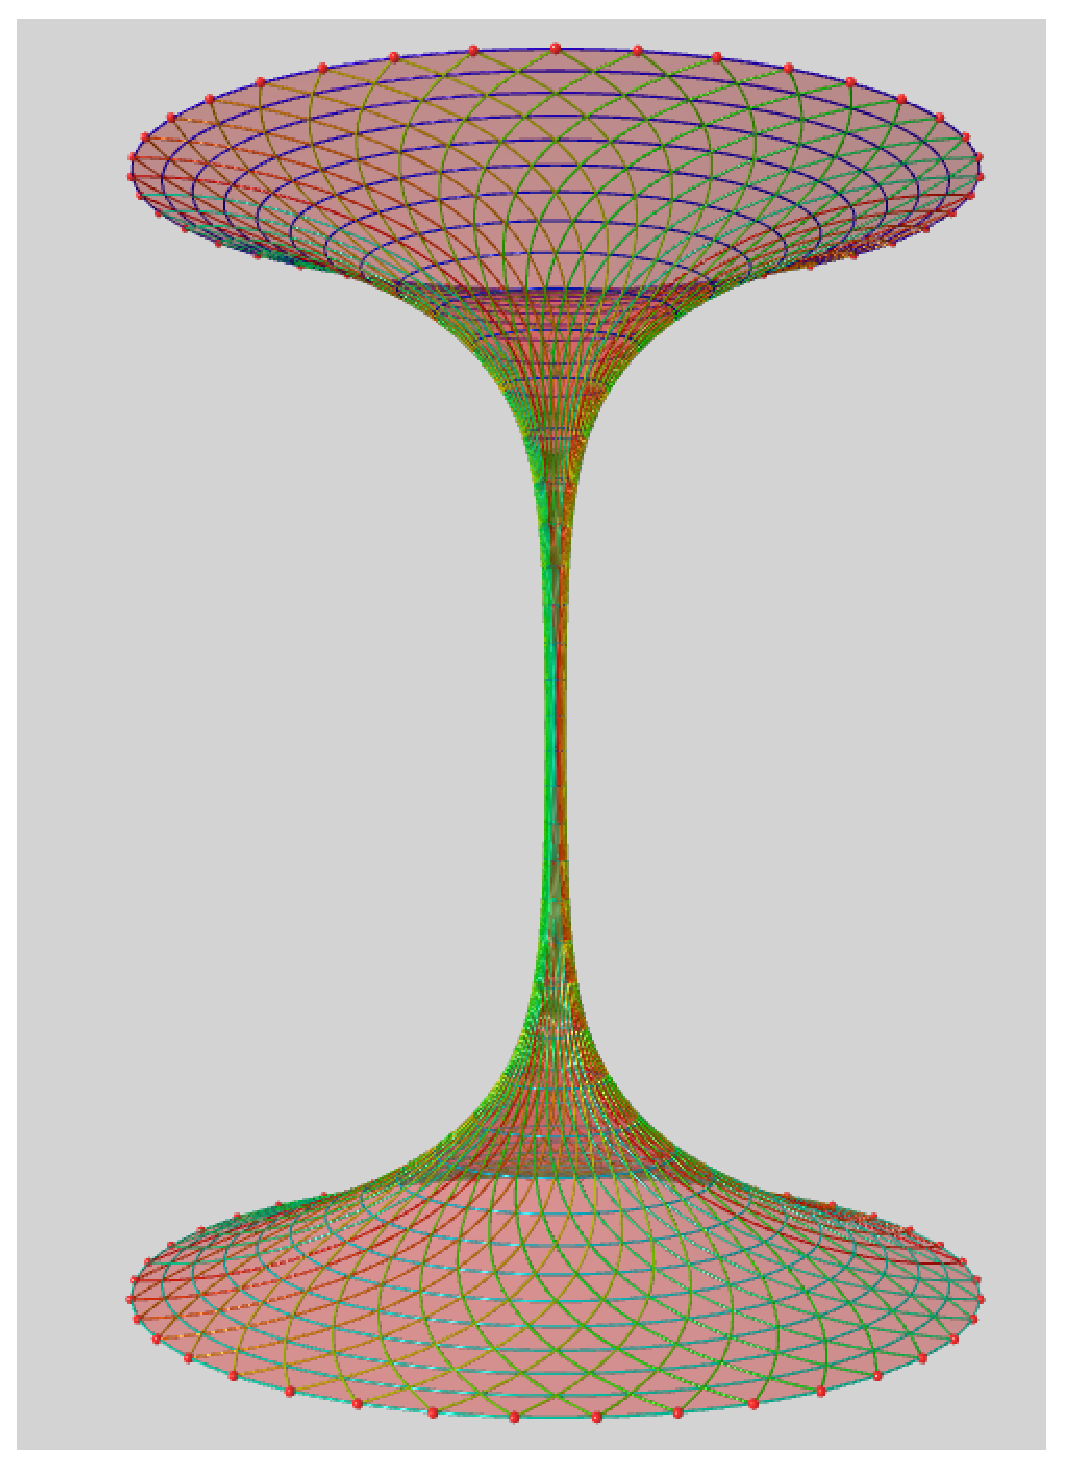
\includegraphics[scale=0.25]{8.eps}
\end{figure}
}
\only<4>{
\begin{figure}[h!]
      \centering 
            \legend{1000 itérations}
      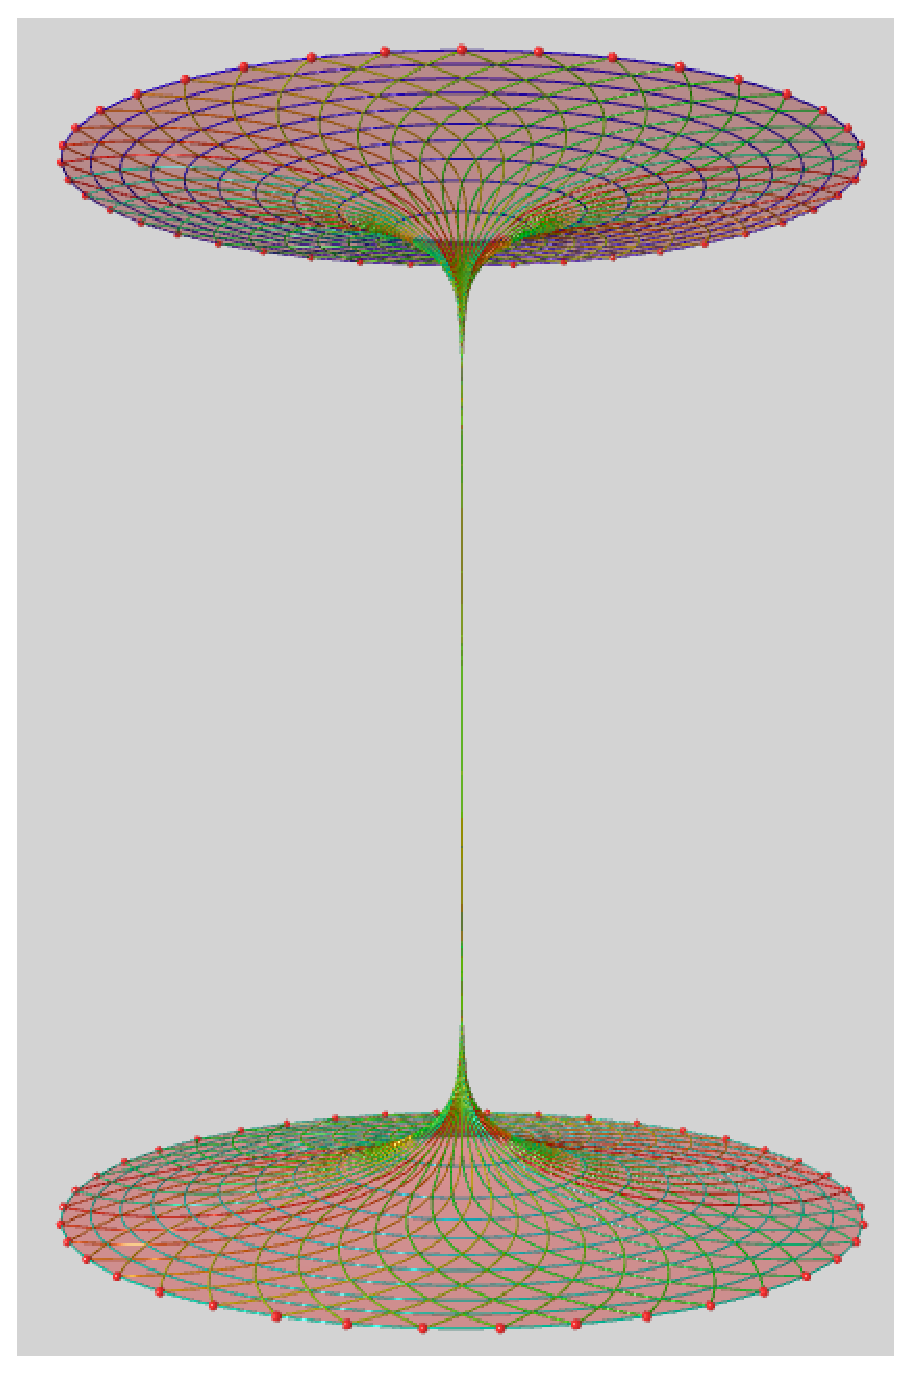
\includegraphics[scale=0.25]{9.eps}
\end{figure}
}
\end{frame}

\subsubsection{Surface de Riemann}

\frame{
\frametitle{Surface de Riemann}
\begin{figure}[ht!]
      \centering 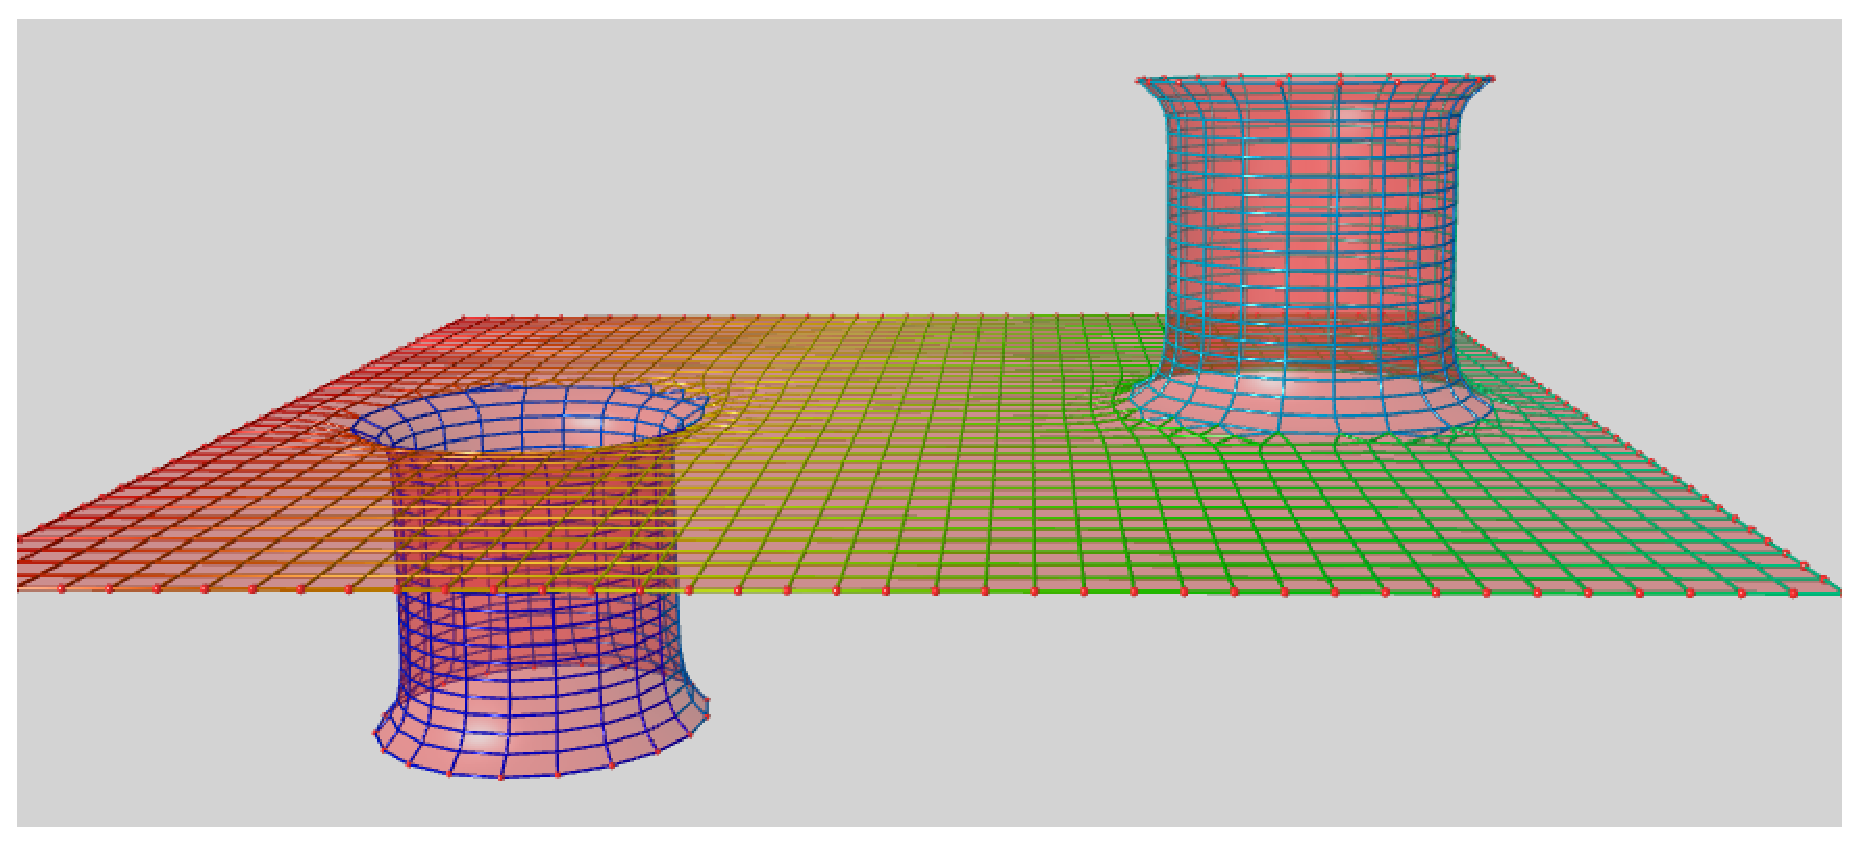
\includegraphics[scale=0.22]{10.eps}
      \legend{Surface de départ}
\end{figure}
\  \vspace{-1cm} \\
\pause
\begin{figure}[ht!]
      \centering 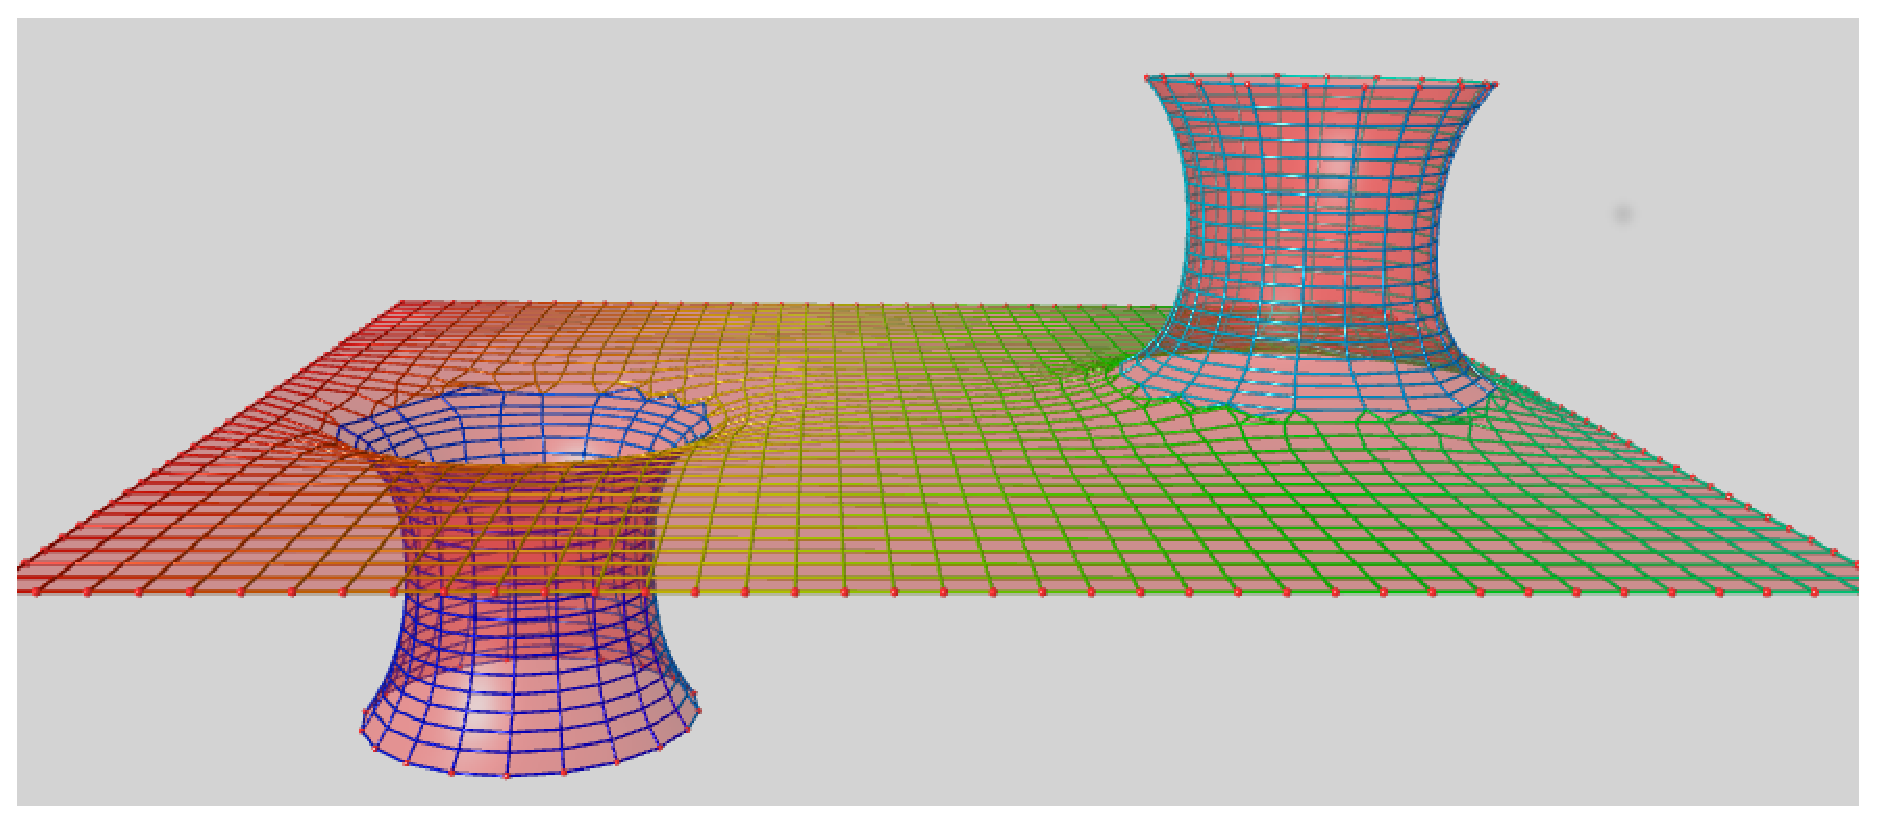
\includegraphics[scale=0.22]{11.eps}
      \legend{Surface finale}
\end{figure}
}

\section{Représentation de Weierstrass}
\subsection{Présentation}

\begin{frame}
\frametitle{Présentation}
$$\Phi(w) = \Re \oint^w \left(
\frac{1}{2}\left(\frac{1}{G}-G\right)h, \frac{i}{2}\left(\frac{1}{G}+G\right)h, h\right) dz $$
\pause
\begin{enumerate}
\item $w\in D$, $D$ est un domaine de $\C$
\item $G$ et $h$ deux fonctions complexes méromorphes sur $D$
\item $Gh$ est holomorphe sur $D$.
\end{enumerate}

$\bullet$ Formule découverte par Weierstrass et Enneper en 1860\\
\pause
$\bullet$ La réciproque est vraie : \\
Toute surface minimale peut s'écrire sous cette forme. 
\end{frame}

\subsection{Implémentation}

\begin{frame}
\frametitle{Implémentation}
$$\Phi(w) = \left(\Re \oint \varphi_1(z), \Re \oint \varphi_2(z), \Re \oint \varphi_3(z)\right), \text{ avec}$$

$$\begin{array}{cc}
\varphi_1(z) = & \frac{1}{2|G|^2}(\overline{G}-\overline{G}G^2)h\\
\varphi_2(z) = & \frac{i}{2|G|^2}(\overline{G}+\overline{G}G^2)h\\
\varphi_3(z) = & h\\
\end{array}
$$
\gs{Entrées} : \\
\begin{itemize}
\item parties réelle et imaginaire de $G$ et $h$
\item un maillage de $D$
\end{itemize}
\end{frame}

\begin{frame}
\frametitle{Intégrale curviligne}
\begin{itemize}
\item $\oint_w^{w'}f(z)dz \approx \frac{f(w)+f(w')}{2}\times (w'-w)$
\item sommet initial $P_0$
\item diviser le maillage $D$ en strates à partir de $P_0$.
\item Relation de Chasles de l'intégrale
\end{itemize}
\begin{figure}[h!]
      \centering 
      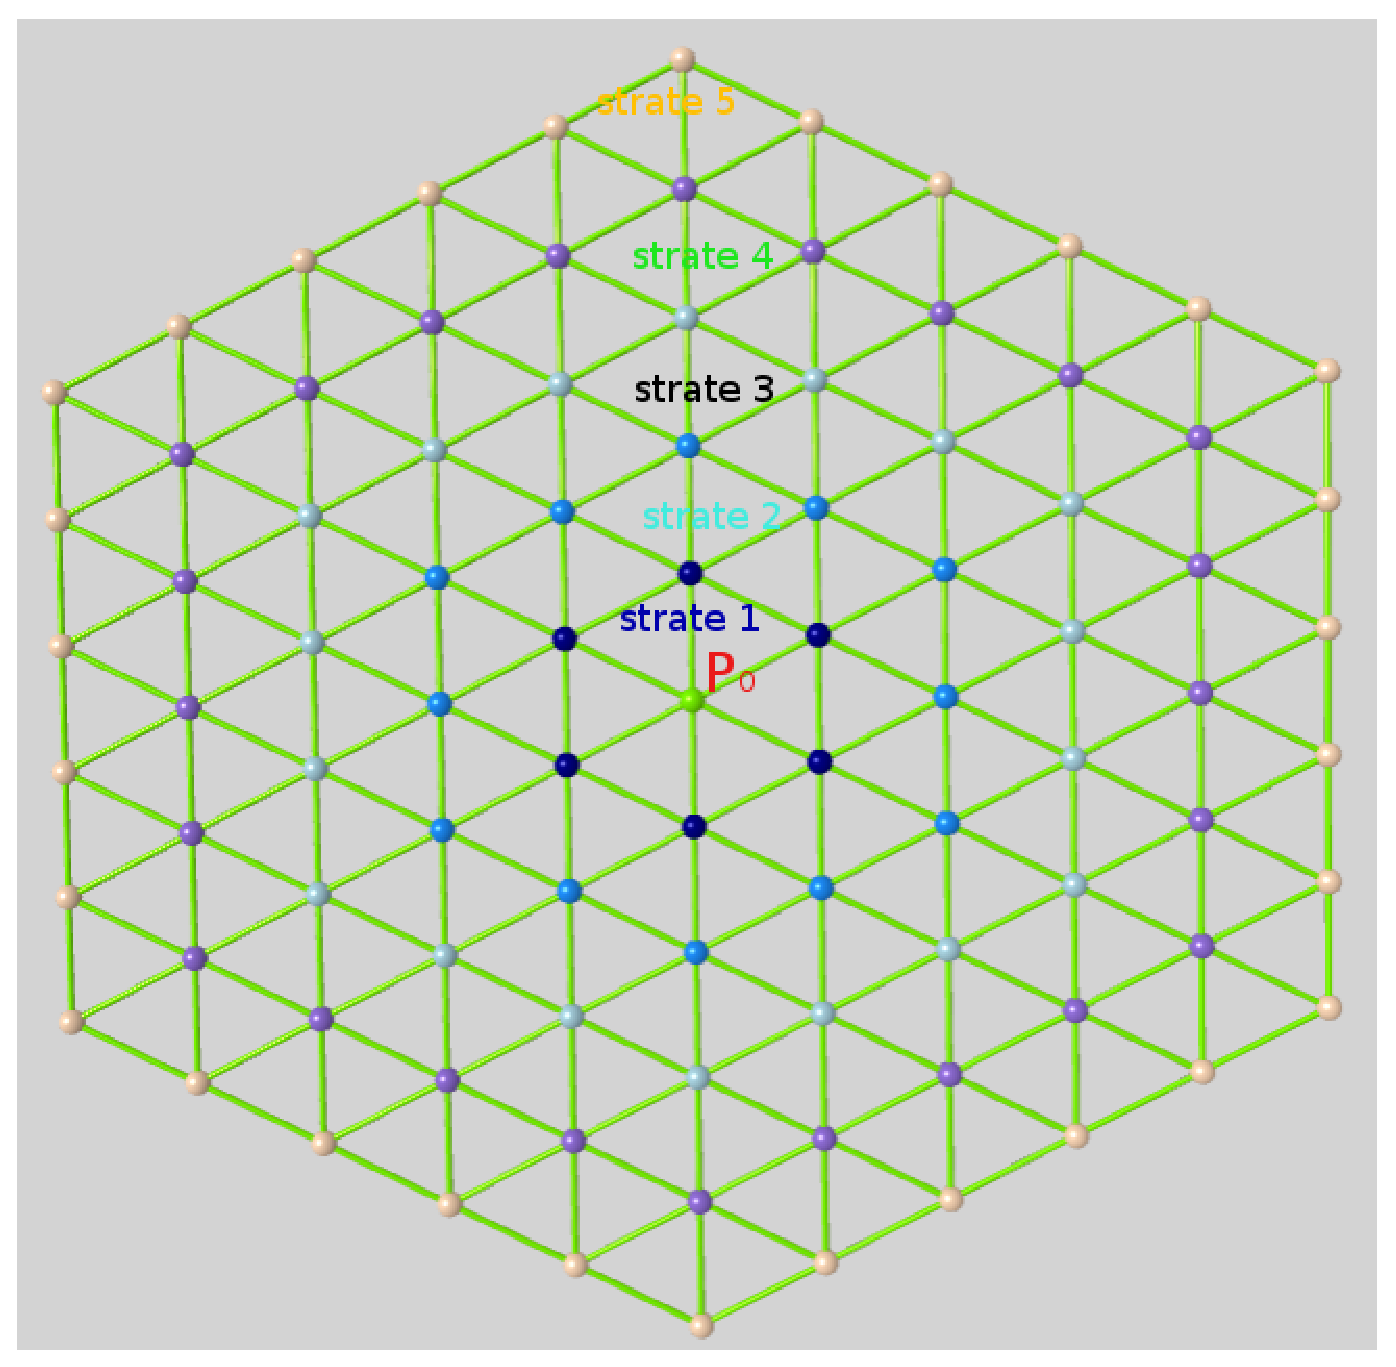
\includegraphics[scale=0.2]{strates.eps}
\end{figure}
\end{frame}

\subsection{Résultats}

\frame{
\frametitle{Maillage de départ}
$\bullet$ Maillage de départ : 
\begin{figure}[h!]
      \centering 
      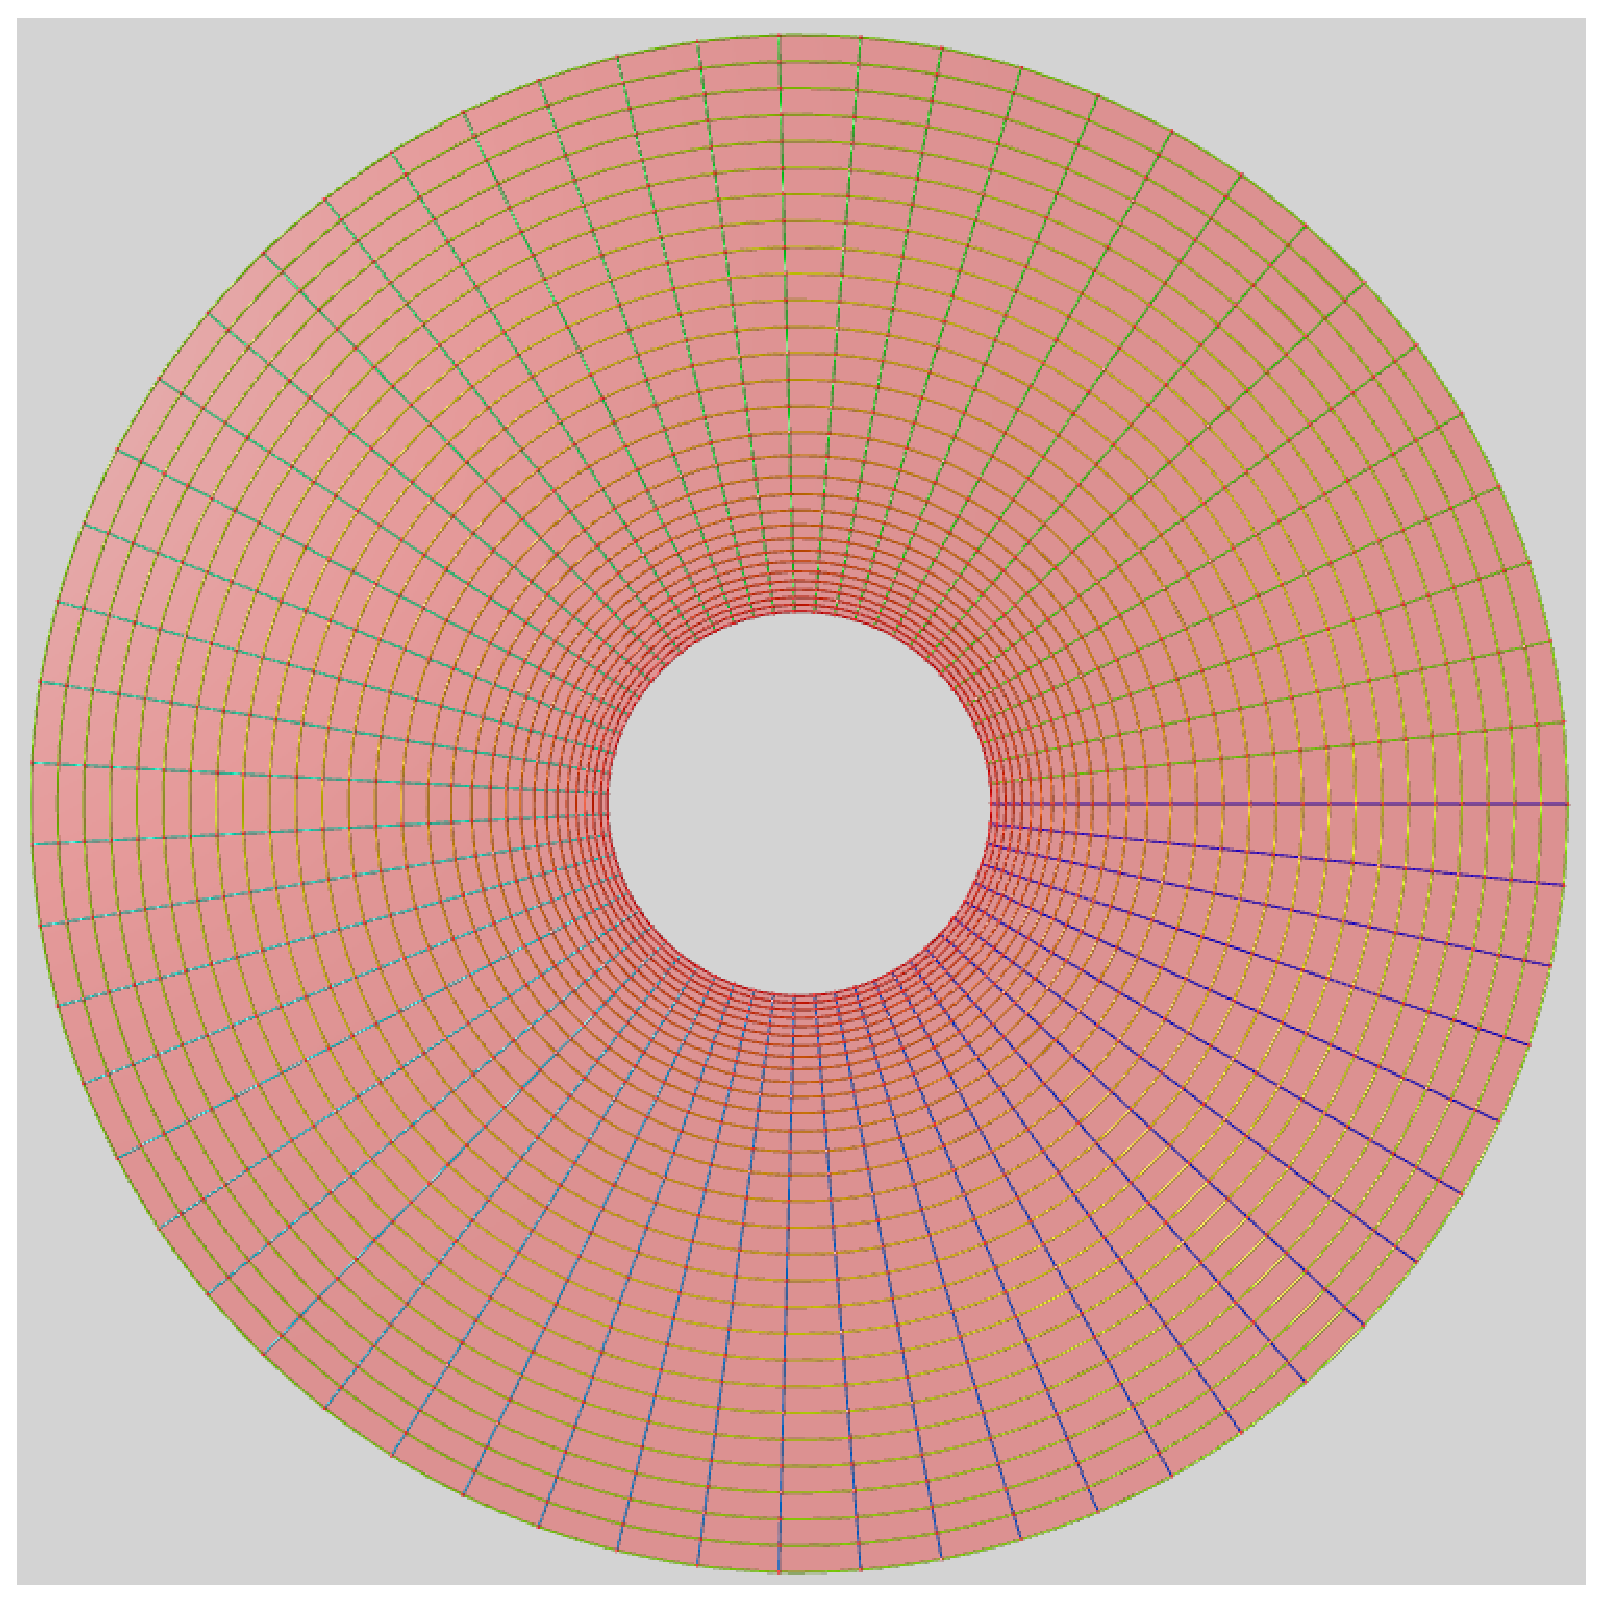
\includegraphics[scale=0.23]{maillageInitial.eps}
\end{figure}
}
\frame{
\frametitle{Le caténoïde}
$G(z)=z$, et $h(z)=\frac{1}{z}$ : 
\begin{figure}[h!]
      \centering 
      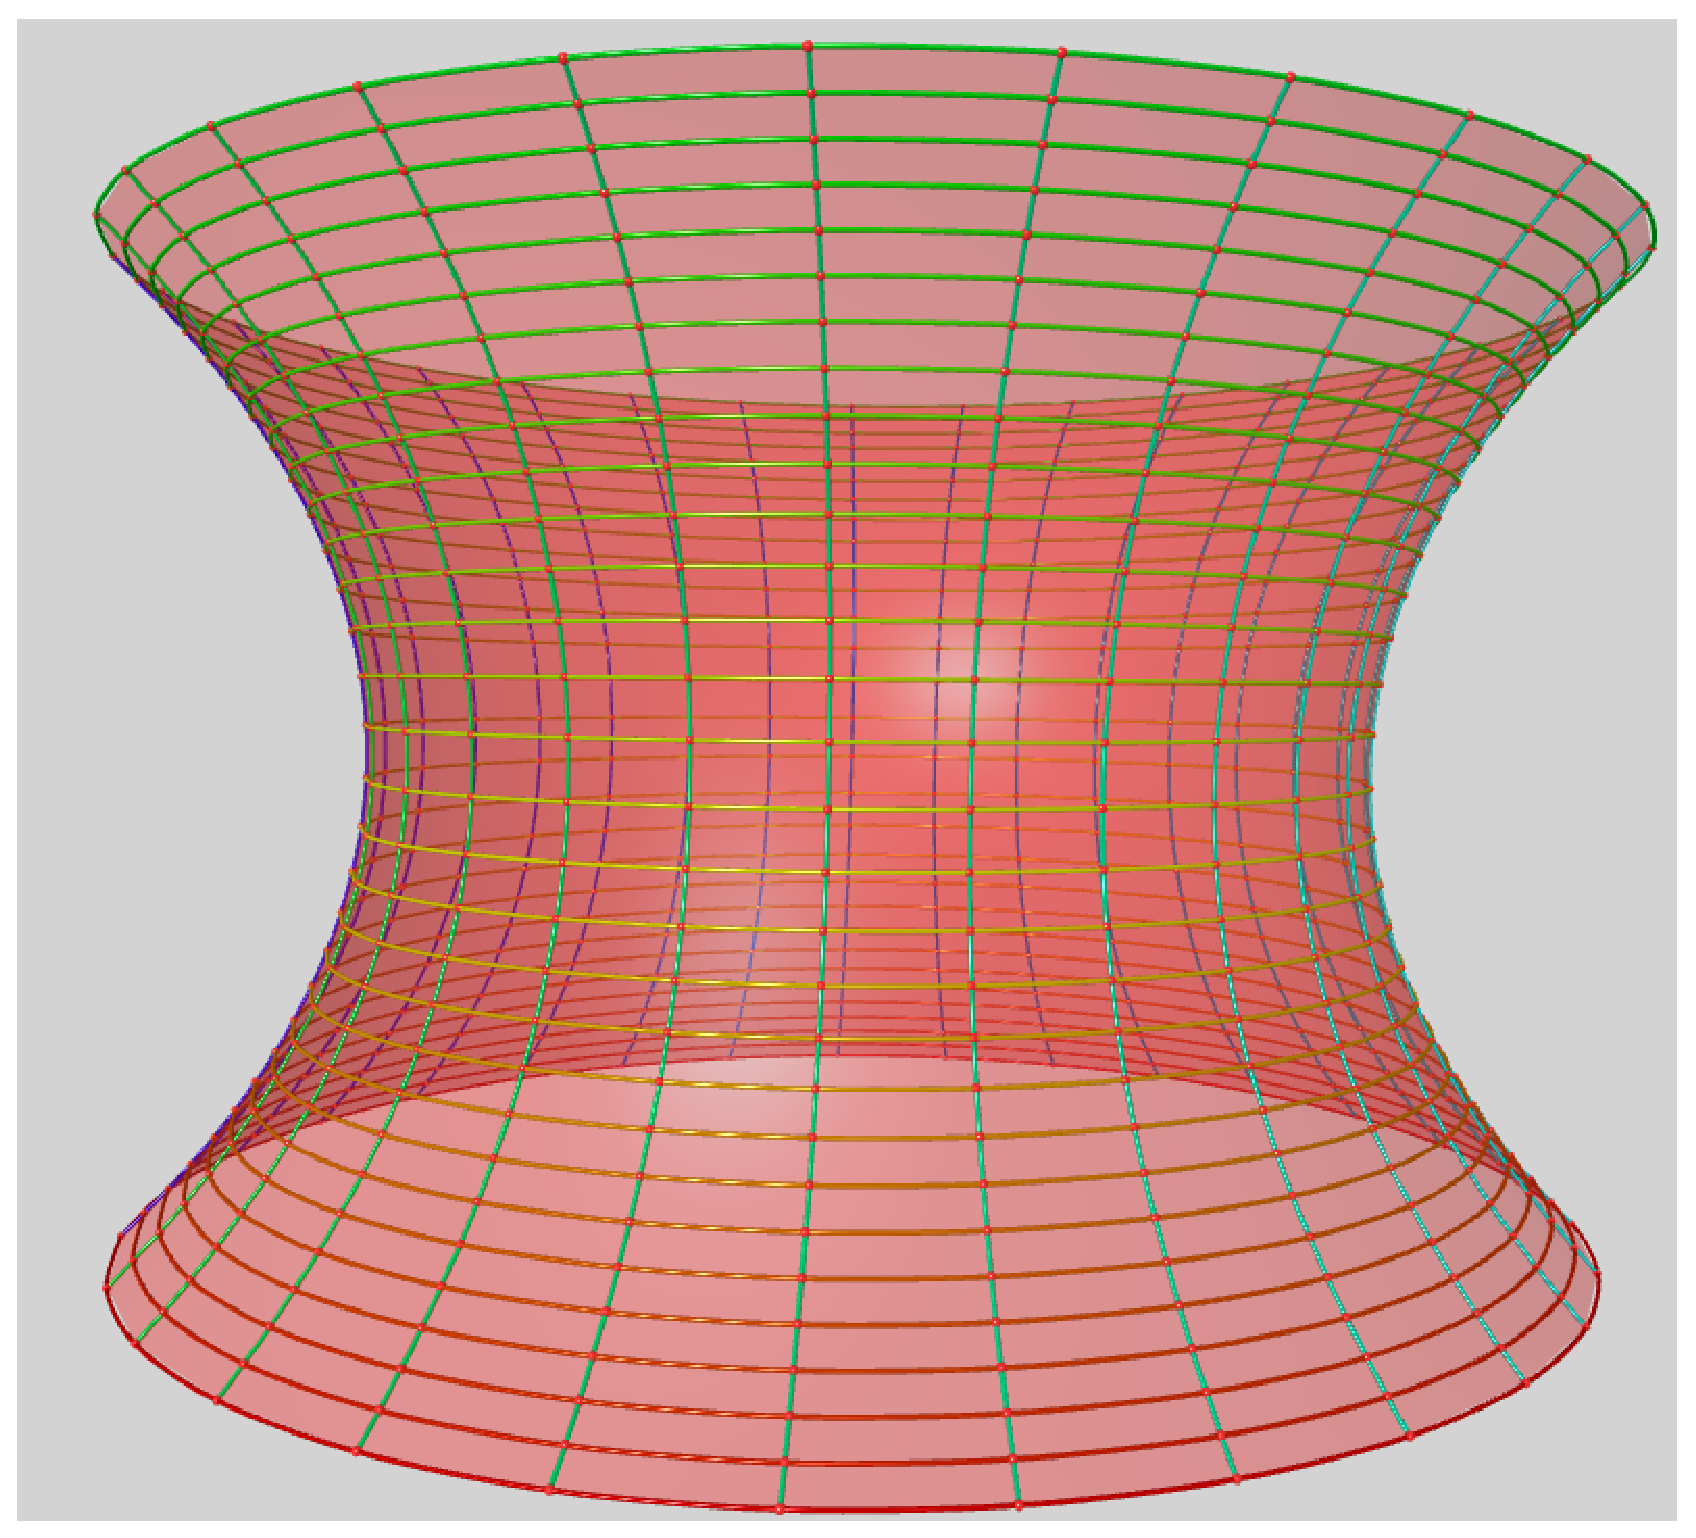
\includegraphics[scale=0.23]{12.eps}
\end{figure}
}

\frame{
\frametitle{L'hélicoïde}
$G(z)=z$, et $h(z)=\frac{i}{z}$ : 

\begin{figure}[h!]
      \centering 
      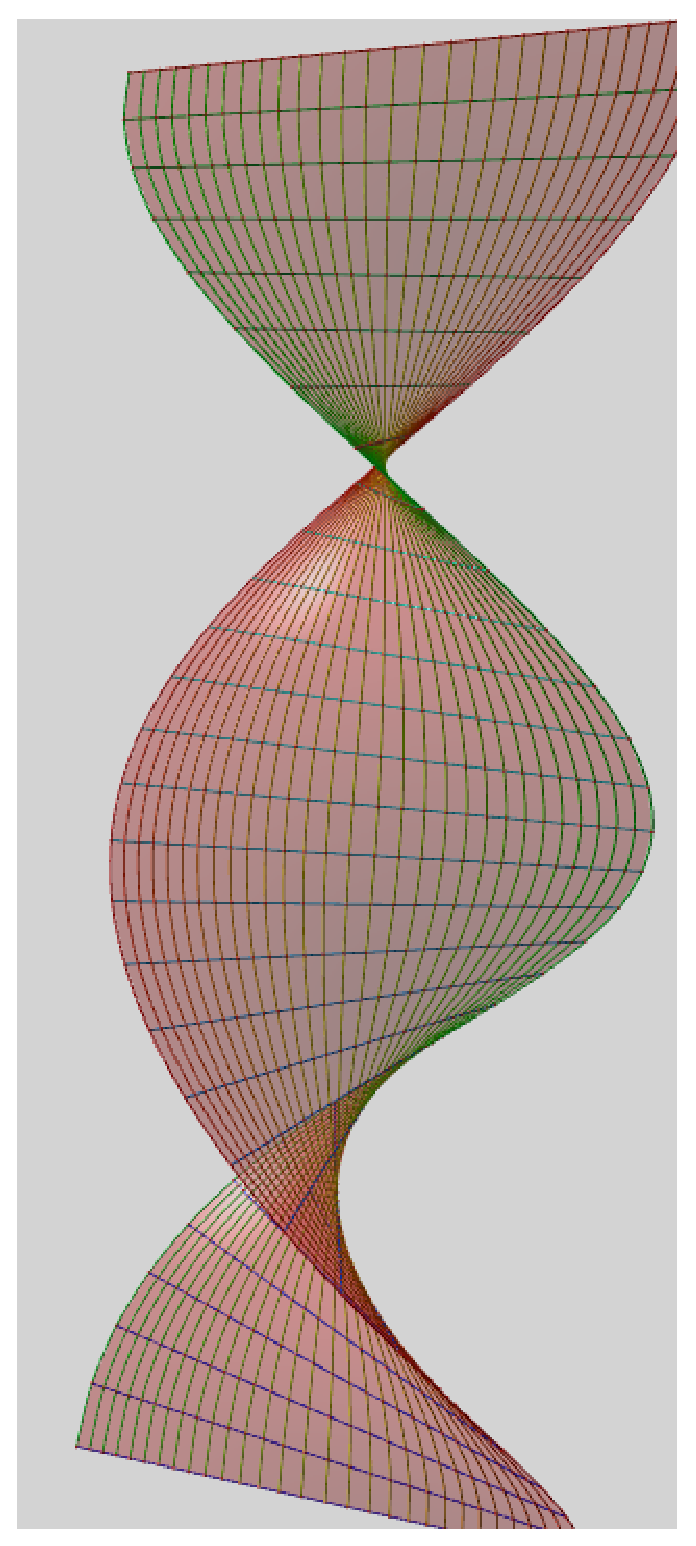
\includegraphics[scale=0.23]{13.eps}
\end{figure}
}

\frame{
\gs{Remarque} :
\begin{itemize}
\item caténoïde : $h_C(z)=\frac{1}{z}$
\item hélicoïde : $h_H(z)=\frac{i}{z}$
\end{itemize}
Ces deux surfaces sont dites \gs{conjuguées}\\
$h_t(z)=e^{t\frac{\pi}{2}}\frac{1}{z},\ t\in [0,1]$ \pause $\Longrightarrow h_0 = h_C$ et $h_1 = h_H$\\
$\Longrightarrow $ Famille de surfaces minimales comprenant la caténoïde et l'hélicoide !
}

\frame{
\frametitle{Surface d'Enneper}
$G(z)=z$, et $h(z)=z$
\begin{figure}[h!]
      \centering 
      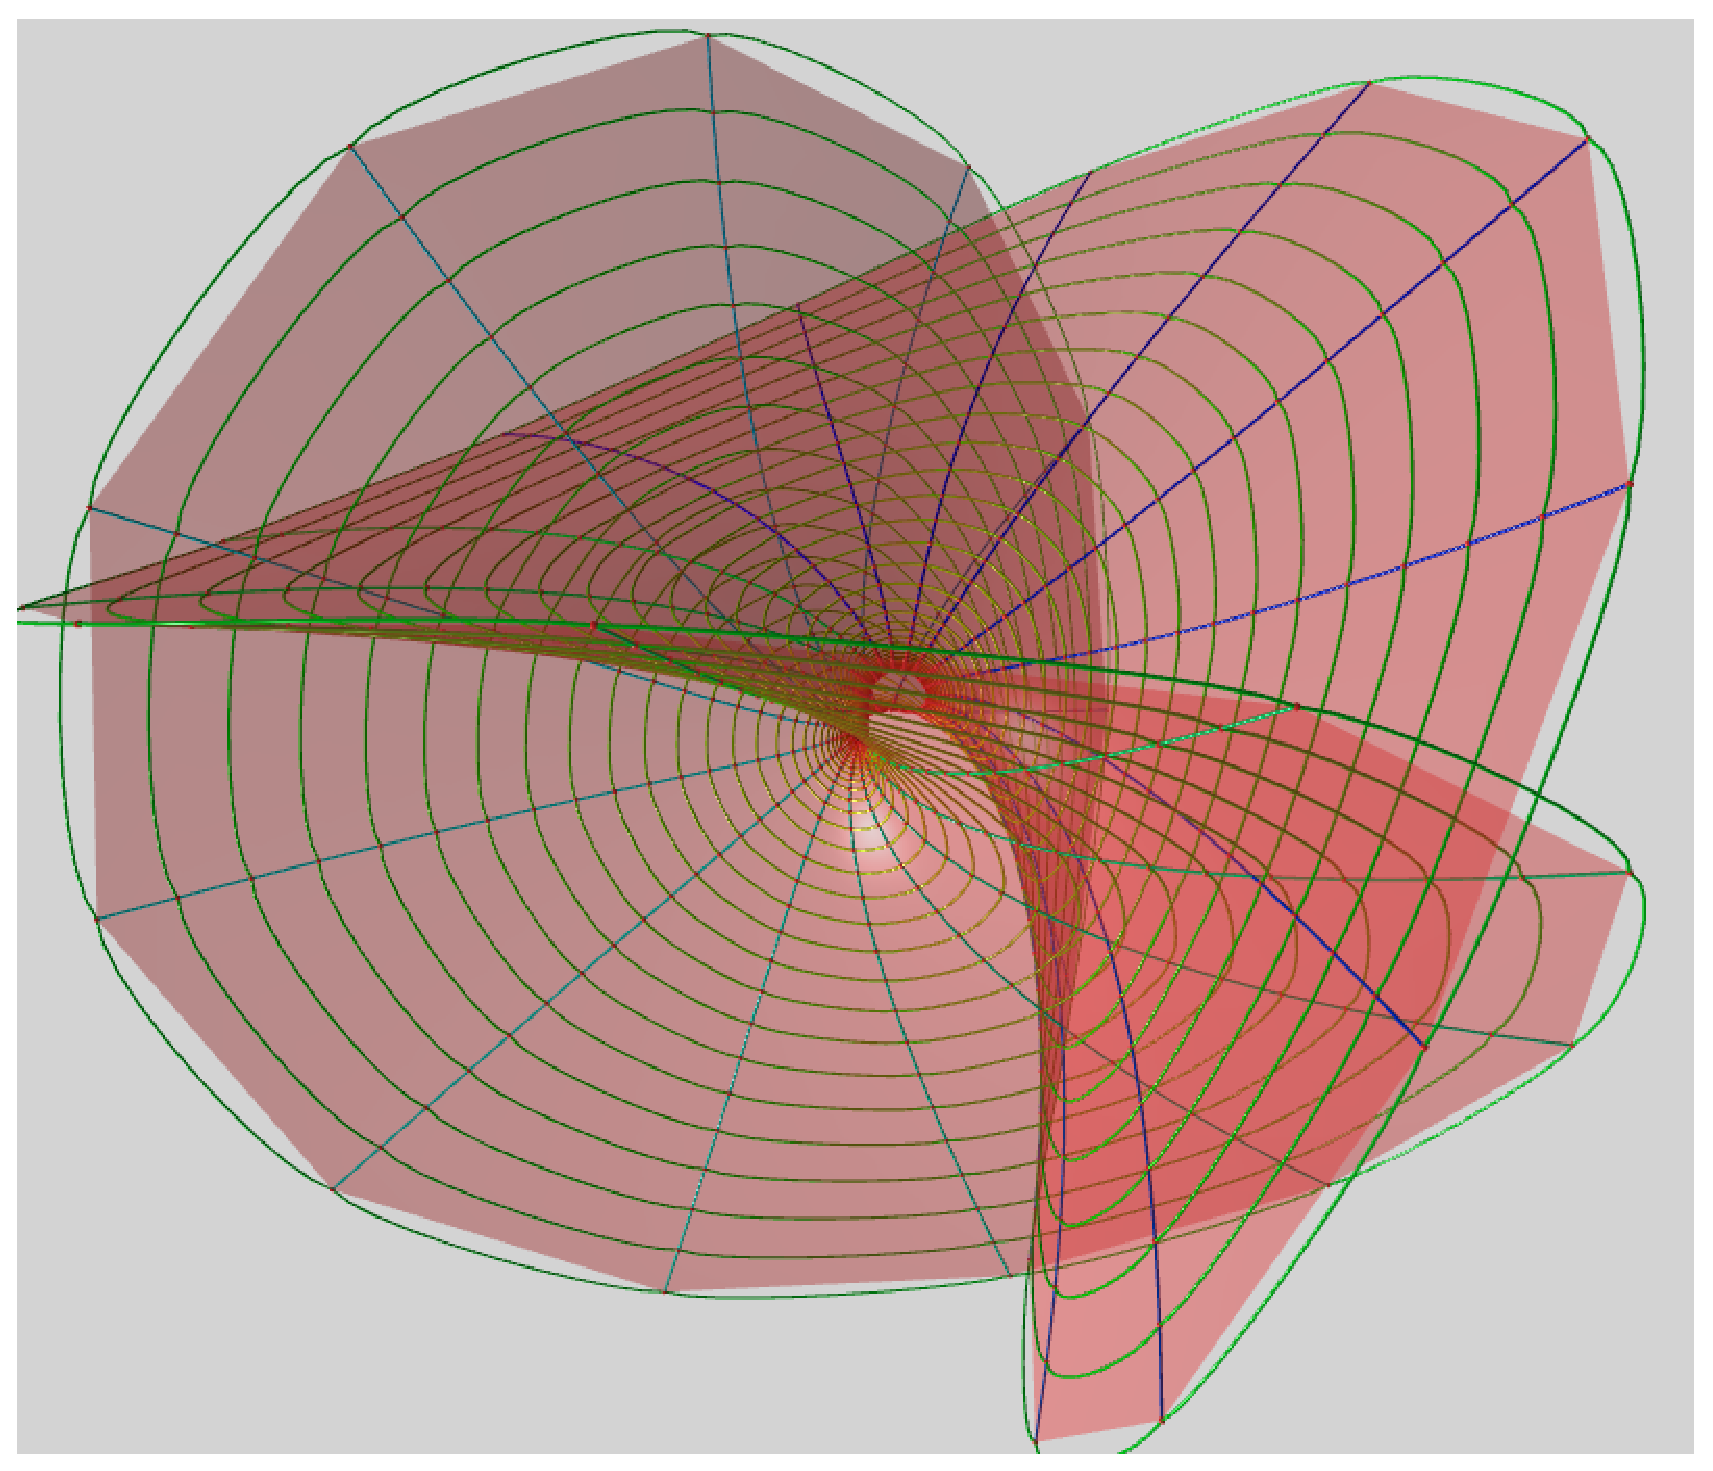
\includegraphics[scale=0.25]{14.eps}
\end{figure}
}

\frame{
\frametitle{Fleur de Jenner}
$G(z)=z$, et $h(z)=z^3$
\begin{figure}[h!]
      \centering 
      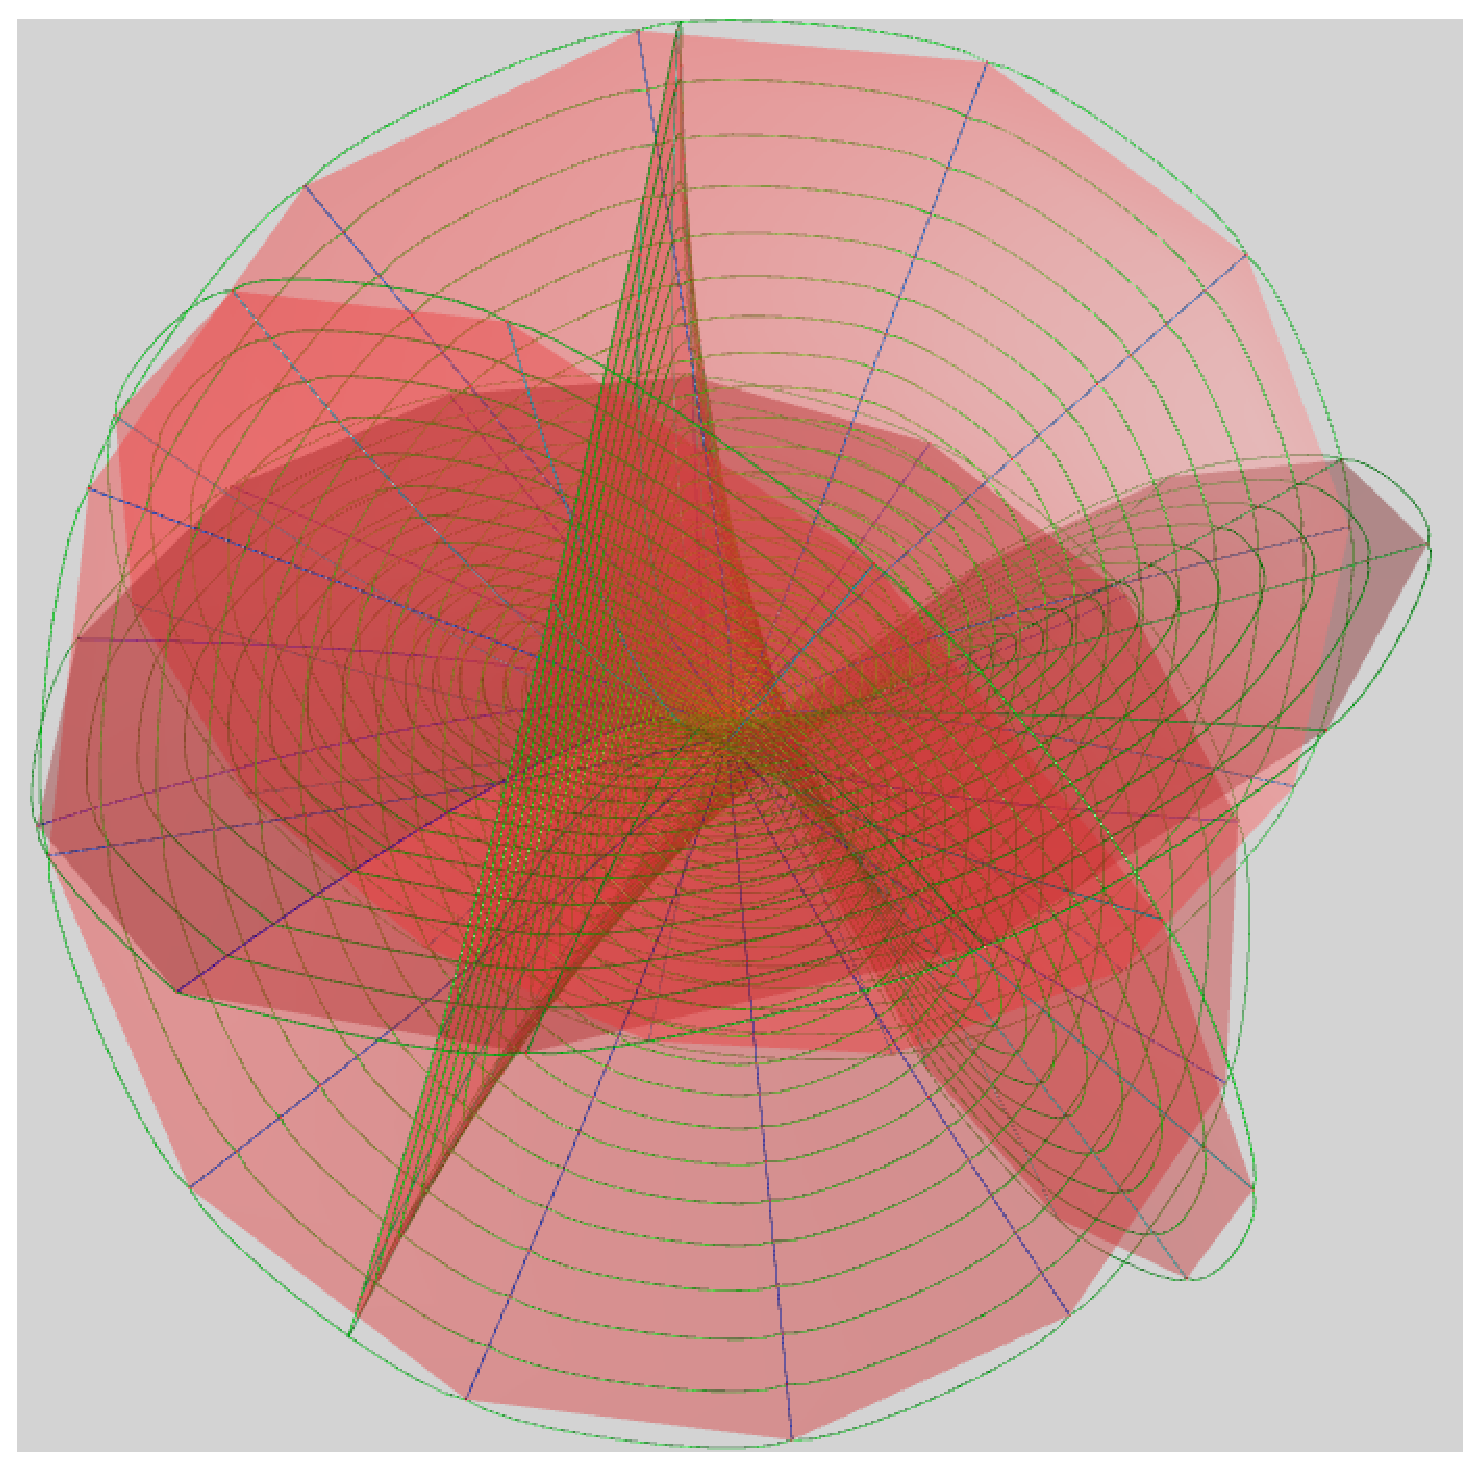
\includegraphics[scale=0.25]{15.eps}
\end{figure}
}

\frame{\textbf{\LARGE Merci pour votre attention !}}

\frame{\gs{Bibliographie}
\begin{itemize}
\item http://www.bridgesmathart.org/art-exhibits/jmm08/sequin.html
\item http://mocosubmit.com/minimal-complexities/
\item Gray A., Modern Differential Geometry of Curves and Surfaces with Mathematica
\item Pinkal U. and Polthier K., Computing Discrete Minimal Surfaces and Their Conjugates
\item Weber M., Classical Minimal Surfaces in Euclidean Space by Examples
\item http://versdusilence.blogspot.fr/2011/03/frei-otto.html
\item https://www.mathcurve.com/surfaces/\\
minimale/minimale.shtml
\end{itemize}
}
\frame{
\begin{itemize}
\item https://www.mathcurve.com/surfaces/\\
catenoid/catenoid.shtml
\item http://images.math.cnrs.fr/Mathematiques-savonneuses.html?lang=fr
\item https://en.wikipedia.org/wiki/\\Minimal\_surface\_of\_revolution
\item https://fr.wikipedia.org/wiki/Surface\_minimale
\item https://en.wikipedia.org/wiki/Enneper\_surface
\item https://fr.wikipedia.org/wiki/Probleme\_de\_Plateau
\end{itemize}
}
\end{document}
